\def\texpath{tex/}
\def\imgpath{images/}
% !TEX option = --shell-escape

\documentclass[a4paper, 10pt, pdftex, twoside=false, numbers=noenddot, fleqn]{scrbook}

	\input{\texpath header}

	\graphicspath{{\imgpath}}
	\addbibresource{bib/articles.bib}

	
\begin{document}

	\input{\texpath titlepage}
	
	\tableofcontents

    \listoffigures
    \newpage

    \listoftables
    \newpage

    \section*{Abkürzungsverzeichnis}
        \begin{tabbing}
    MAG \hspace{1cm} \= Mitarbeitergespräch \\
    API \> Application Programming Interface \\
    JSON \> JavaScript Object Notation \\
    3D \> Dreidimensional
         \end{tabbing}
    \newpage


	\chapter{Einleitung} \label{chap:einleitung}

Die Qualität und Effizienz von Mitarbeitendengesprächen sind essenziell für den Erfolg eines Unternehmens. Solche Gespräche schaffen eine Plattform für Feedback, Leistungsbewertungen, die gemeinsame Festlegung von Zielen und die Planung individueller Entwicklungsmöglichkeiten. Regelmäßige  Gespräche tragen nicht nur zur Stärkung der Mitarbeitendenbindung bei, sondern fördern auch die Produktivität und die strategische Ausrichtung des Unternehmens, indem sie die Ziele der Organisation mit den Bedürfnissen der Mitarbeitenden in Einklang bringen \cite{Schober2008, Bryson2011}.

In einer zunehmend datengetriebenen Welt wird es immer wichtiger, große Datenmengen nicht nur zu sammeln, sondern auch sinnvoll zu nutzen. Gerade im Bereich Human Resources (\hyperref[abkuerzungen]{HR}) bleiben die Ergebnisse von Mitarbeitendengesprächen oft ungenutzt, da sie in unstrukturierter Form vorliegen. Dadurch entgehen Unternehmen wertvolle Einblicke, die zur Förderung der Mitarbeitendenentwicklung und zur Optimierung von HR-Strategien beitragen könnten \cite{Kirk2016}. Der Einsatz moderner Visualisierungstools bietet hier eine Lösung, indem er die Darstellung und Analyse solcher Daten erleichtert und datenbasierte Entscheidungen unterstützt.

Trotz der zunehmenden Digitalisierung in Unternehmen existiert eine Forschungslücke in der Verbindung zwischen datengetriebener Analyse und der praktischen Umsetzung in Mitarbeitendengesprächen. Während Studien die Vorteile datenbasierter Ansätze im (\hyperref[abkuerzungen]{HR})-Management betonen \cite{Evergreen2016}, fehlen praxisnahe Beispiele, die moderne Technologien wie interaktive Visualisierungen und cloudbasierte Datenverarbeitung zur Optimierung solcher Gespräche nutzen. Diese Arbeit schließt diese Lücke, indem sie ein System entwickelt, das datengetriebene Erkenntnisse für Mitarbeitendengespräche praktisch anwendbar macht.

Die Inhalte der Arbeit wurden in Zusammenarbeit mit der Realcore Services GmbH entwickelt, einem führenden IT-Dienstleister, der sich auf innovative Lösungen für die Optimierung interner Prozesse spezialisiert hat. Ziel der Arbeit ist es, ein modernes und benutzerfreundliches Reporting-Tool zu entwickeln, das speziell für die Analyse und Visualisierung von Daten aus Mitarbeitendengesprächen konzipiert ist. Dabei werden technologische Ansätze wie React, .NET Core und Microsoft Azure eingesetzt, um eine flexible, skalierbare und sichere Plattform zu schaffen.

Die zentrale Forschungsfrage dieser Arbeit lautet: \begin{quote} Wie können datenbasierte Visualisierungen und moderne Technologien zur Optimierung von Mitarbeitendengesprächen beitragen und deren Effizienz sowie strategische Relevanz für Unternehmen erhöhen? \end{quote}

Wissenschaftlich leistet diese Arbeit einen Beitrag zur Integration von datengetriebenen Visualisierungen und modernen Technologien in den Kontext von Mitarbeitendengesprächen. Sie untersucht nicht nur die technische Machbarkeit solcher Systeme, sondern auch die Akzeptanz und Praxistauglichkeit in der realen Arbeitswelt. Dadurch liefert sie wertvolle Erkenntnisse für zukünftige Forschung und Entwicklung in diesem Bereich.

Die zentralen Herausforderungen liegen dabei in der effizienten Verarbeitung von Daten aus Mitarbeitendengesprächen, die oft in fragmentierter oder unstrukturierter Form vorliegen. Ziel ist es, diese Daten zu organisieren und durch interaktive Visualisierungen wie Donut-Diagramme und Radarcharts zugänglich zu machen, um Führungskräfte und (\hyperref[abkuerzungen]{HR})-Abteilungen bei der Entscheidungsfindung zu unterstützen \cite{Evergreen2016}. Neben der technischen Umsetzung wird auch untersucht, wie das entwickelte System durch benutzerzentrierte Gestaltung Akzeptanz und Praxistauglichkeit erhöhen kann.

Die vorliegende Arbeit gliedert sich wie folgt: Im Kapitel~\ref{chap:theoretische-grundlagen} werden die theoretischen Grundlagen vorgestellt, die die Bedeutung von Mitarbeitendengesprächen, die Rolle der Datenvisualisierung und die eingesetzten Technologien umfassen. Kapitel~\ref{chap:analysephase} widmet sich der Analyse der Anforderungen durch Stakeholder-Interviews und einen Vergleich bestehender Lösungen. Die Konzeption des Systems, einschließlich der Systemarchitektur, des Datenmodells und der Sicherheitsmaßnahmen, wird im Kapitel~\ref{chap:konzeption} beschrieben. Kapitel~\ref{chap:implementierung} behandelt die technische Implementierung, wobei auf Herausforderungen und deren Lösungen eingegangen wird. Im Kapitel~\ref{chap:evaluation} wird das System evaluiert, indem Funktionstests und Usability-Analysen durchgeführt werden. Abschließend fasst Kapitel~\ref{chap:fazit} die Ergebnisse zusammen und gibt einen Ausblick auf mögliche Weiterentwicklungen.

Diese Arbeit soll insgesamt nicht nur zur Effizienzsteigerung von Mitarbeitendengesprächen beitragen, sondern auch zeigen, wie datenbasierte Ansätze die strategische Ausrichtung und Entscheidungsfindung in Unternehmen nachhaltig unterstützen können. Darüber hinaus liefert sie praktische Erkenntnisse, wie innovative Technologien die Digitalisierung von (\hyperref[abkuerzungen]{HR})-Prozessen vorantreiben können.
	\chapter{Theoretische Grundlagen}
\label{chap:theoretische-grundlagen}

Die individuelle Entwicklung von Mitarbeitenden erfolgt maßgeblich durch zielgerichtete Gespräche und datengestützte Feedbackprozesse. Die folgenden Abschnitte beleuchten die Bedeutung von Mitarbeitendengesprächen, die Rolle der Datenvisualisierung in diesem Kontext sowie die technologische Basis für deren Implementierung. Hierbei wird auf die Verknüpfung von strategischen Unternehmenszielen und persönlichen Entwicklungsmöglichkeiten eingegangen, um eine nachhaltige Verbesserung der Teamdynamik und Leistungseffizienz zu fördern. Diese theoretischen Grundlagen bilden das Fundament für die anschließende Analyse und Entwicklung eines optimalen Systems zur Visualisierung von Mitarbeitendengesprächsdaten.

\section{Mitarbeitendengespräche und ihre Bedeutung}
Mitarbeitendengespräche, auch als „MAG“ bezeichnet, umfassen alle Gespräche, die Vorgesetzte mit Mitarbeitenden zu spezifischen Anlässen führen. Diese Gespräche dienen dazu:
\begin{itemize}
    \item Informationen auszutauschen,
    \item Wertschätzung, Lob oder Kritik zu äußern und
    \item Entwicklungsziele zu formulieren \cite{schober2008}.
\end{itemize}

Ein strukturierter Ablauf solcher Gespräche fördert die innerbetriebliche Kommunikation und die Bindung der Mitarbeitenden an das Unternehmen. Typische Elemente von Mitarbeitendengesprächen sind:
\begin{itemize}
    \item \textbf{Bewertung der bisherigen Zielerreichung:} Analyse des Fortschritts in Bezug auf zuvor gesetzte Ziele \cite{duarte2012performance}.
    \item \textbf{Setzen neuer Ziele:} Definition von SMART-Zielen (spezifisch, messbar, akzeptiert, realistisch, terminiert), die eine klare Richtung für die zukünftige Arbeit vorgeben \cite{duarte2012performance}.
    \item \textbf{Diskussion von Entwicklungsmaßnahmen:} Identifikation von Schulungsbedarf und Weiterbildungsangeboten zur Förderung von persönlichem und beruflichem Wachstum \cite{bryson2011employee}.
\end{itemize}

Eine strukturierte Gesprächsführung kann Verzerrungen durch subjektive Einschätzungen minimieren, insbesondere durch den Einsatz datenbasierter Methoden \cite{heikkila2018}. Dies unterstützt Führungskräfte dabei, fundierte Entscheidungen zu treffen, die sowohl die individuellen Ziele der Mitarbeitenden als auch die strategischen Unternehmensziele berücksichtigen \cite{barton2012}.

\section{Relevanz von Datenvisualisierung}
Datenvisualisierung ist ein zentraler Bestandteil moderner Analytik und spielt eine entscheidende Rolle bei der Interpretation komplexer Informationen. Sie unterstützt Führungskräfte dabei, datenbasierte Entscheidungen zu treffen, indem sie große Datenmengen in verständliche visuelle Darstellungen umwandelt \cite{kirk2016data}. 

\subsection*{Hauptvorteile der Datenvisualisierung}
\begin{itemize}
    \item \textbf{Verbesserte Entscheidungsfindung:} Daten werden schneller und effizienter interpretiert \cite{kirk2016data}.
    \item \textbf{Erkennung von Trends und Abweichungen:} Historische und aktuelle Daten können leicht verglichen werden, um Entwicklungen zu identifizieren \cite{ware2012information}.
    \item \textbf{Kommunikation und Präsentation:} Visualisierte Daten fördern eine klare Kommunikation zwischen Teams und Stakeholdern \cite{evergreen2016effective}.
\end{itemize}

Im Kontext von Mitarbeitendengesprächen sind Radarcharts und Donutcharts besonders geeignet:
\begin{itemize}
    \item \textbf{Radarcharts:} Vergleich mehrerer Leistungsdimensionen wie Teamarbeit, Effizienz und Pünktlichkeit \cite{heikkila2018}.
    \item \textbf{Donutcharts:} Übersicht über den Status von Zielvereinbarungen oder Fortschritten \cite{evergreen2016effective}.
\end{itemize}
\newpage

\section{Technologische Basis}
Die technologische Basis für ein System zur Visualisierung von Mitarbeitendengesprächsdaten ist entscheidend für dessen Funktionalität, Benutzerfreundlichkeit und Skalierbarkeit. Die ausgewählten Technologien umfassen:

\begin{itemize}
    \item \textbf{React:} Eine JavaScript-Bibliothek für die komponentenbasierte Entwicklung dynamischer Benutzeroberflächen \cite{stefanov2021react}.
    \item \textbf{TypeScript:} Erweiterung von JavaScript mit statischer Typisierung zur Verbesserung der Codequalität \cite{typeScriptDocumentation}.
    \item \textbf{.NET Core:} Plattformübergreifendes Framework für die Entwicklung skalierbarer und leistungsstarker Backend-Anwendungen \cite{microsoftDotNet}.
    \item \textbf{MSSQL:} Eine cloudbasierte Datenbanklösung, die Sicherheit und Skalierbarkeit für große Datenmengen bietet \cite{azureDocumentation}.
    \item \textbf{Azure Ressourcen:} Verschiedene Dienste von Microsoft Azure wurden in der Implementierung genutzt, um eine umfassende und skalierbare Lösung zu gewährleisten:
    \begin{itemize}
       \item \textbf{Entra ID (ehemals Azure Active Directory):} Entra ID bietet umfassende Authentifizierungs- und Autorisierungsdienste, einschließlich Multi-Faktor-Authentifizierung und rollenbasierter Zugriffskontrolle. Studien zeigen, dass die Verwendung solcher Systeme die Sicherheit und Effizienz in Unternehmen erheblich erhöht \cite{microsoftEntraID, woods2020authentication}.
\item \textbf{Microsoft Graph API:} Diese API ermöglicht die Interaktion mit verschiedenen Microsoft-Diensten, wie Benutzerdatenabfragen und Kalenderintegration. Laut aktuellen Forschungsergebnissen ist die Nutzung von Graph APIs ein Schlüssel für die Automatisierung und Integration in moderne Softwarelandschaften \cite{microsoftGraphAPI, smith2021graph}.
\item \textbf{Application Insights:} Ein Telemetriedienst, der zur Überwachung und Analyse der Anwendungsleistung eingesetzt wird. Studien belegen, dass Application Insights eine signifikante Verbesserung in der Fehlerdiagnose und Performanceanalyse moderner Cloud-Anwendungen ermöglicht \cite{microsoftAppInsights, li2021monitoring}.
\item \textbf{App Services:} Ein Telemetriedienst, der zur Überwachung und Analyse der Anwendungsleistung eingesetzt wird. Studien belegen, dass Application Insights eine signifikante Verbesserung in der Fehlerdiagnose und Performanceanalyse moderner Cloud-Anwendungen ermöglicht 
\item \textbf{Container Registry:} Ein Telemetriedienst, der zur Überwachung und Analyse der Anwendungsleistung eingesetzt wird. Studien belegen, dass Application Insights eine signifikante Verbesserung in der Fehlerdiagnose und Performanceanalyse moderner Cloud-Anwendungen ermöglicht 

\end{itemize}

\item \textbf{Git:} Verschiedene Dienste von Microsoft Azure wurden in der Implementierung genutzt, um eine umfassende und skalierbare Lösung zu gewährleisten
\item \textbf{DevOps:} Verschiedene Dienste von Microsoft Azure wurden in der Implementierung genutzt, um eine umfassende und skalierbare Lösung zu gewährleisten:
    \begin{itemize}    
    \item \textbf{CI/CD-Pipeline:} Mit Azure DevOps werden automatisierte Continuous Integration und Continuous Deployment (CI/CD) umgesetzt, um Entwicklungs- und Bereitstellungsprozesse zu optimieren. Aktuelle Veröffentlichungen zeigen, dass CI/CD-Pipelines die Bereitstellungszeit um bis zu 50 \% reduzieren können \cite{azureDevOps, fowler2020continuous}.
     \item \textbf{HBS-Masstransit Artefakt:} Mit Azure DevOps werden automatisierte Continuous Integration und Continuous Deployment (CI/CD) umgesetzt, um Entwicklungs- und Bereitstellungsprozesse zu optimieren. Aktuelle Veröffentlichungen zeigen, dass CI/CD-Pipelines die Bereitstellungszeit um bis zu 50 \% reduzieren können \cite{azureDevOps, fowler2020continuous}.

      \item \textbf{Repository:} Mit Azure DevOps werden automatisierte Continuous Integration und Continuous Deployment (CI/CD) umgesetzt, um Entwicklungs- und Bereitstellungsprozesse zu optimieren. Aktuelle Veröffentlichungen zeigen, dass CI/CD-Pipelines die Bereitstellungszeit um bis zu 50 \% reduzieren können \cite{azureDevOps, fowler2020continuous}.
\end{itemize}


\subsection*{Integration der Technologien}
Die Kombination aus React und TypeScript ermöglicht die Entwicklung einer flexiblen und responsiven Benutzeroberfläche. Backend-seitig sorgt .NET Core für eine skalierbare und performante Architektur, während MS SQL als sichere Speicherlösung dient. Die enge Verzahnung dieser Technologien gewährleistet eine effiziente Datenverarbeitung und nahtlose Integration in bestehende Infrastrukturen \cite{microsoftAzure}.

\section{Zusammenfassung}
Mitarbeitendengespräche, unterstützt durch Datenvisualisierung und moderne Technologien, bieten erhebliches Potenzial zur Förderung der Teamdynamik und zur Erreichung von Unternehmenszielen. Die theoretischen Grundlagen zeigen, dass die Kombination von strukturierten Gesprächen, datenbasierter Entscheidungsfindung und technologischen Innovationen die Basis für ein effizientes und skalierbares System bildet.


	\chapter{Analysephase}
\label{chap:analysephase}

\section{Anforderungen}
\subsection{Funktionale Anforderungen}
Das geplante Tool soll den spezifischen Anforderungen der Zielgruppe gerecht werden und folgende Funktionen umfassen:
\begin{itemize}
    \item \textbf{Visualisierung:} Darstellung der Gesprächsdaten als Donut- und Radarcharts. Diese Diagramme ermöglichen eine schnelle Erfassung von Trends und Leistungskennzahlen und sind besonders geeignet, um die Ergebnisse von Mitarbeitendengesprächen verständlich zu präsentieren \cite{kirk2016data, evergreen2016effective}.
    \item \textbf{Datenmanagement:} Import, Speicherung und Bearbeitung von Gesprächsdaten. Diese Funktion gewährleistet eine strukturierte Datenverwaltung und unterstützt die Nachverfolgbarkeit vergangener Gespräche \cite{bryson2011employee}.
    \item \textbf{Export:} Generierung von Berichten im Excel- und PDF-Format, die Führungskräfte für weitere Analysen oder Präsentationen nutzen können.
    \item \textbf{Benutzerverwaltung:} Rollenspezifischer Zugriff (z. B. Admins, Führungskräfte), um sicherzustellen, dass nur berechtigte Personen auf sensible Daten zugreifen können \cite{duarte2012performance}.
\end{itemize}

\subsection{Nicht-funktionale Anforderungen}
Neben den funktionalen Anforderungen sind nicht-funktionale Kriterien von entscheidender Bedeutung, um die Qualität und Effizienz des Tools sicherzustellen:
\begin{itemize}
    \item \textbf{Performance:} Schnelle Verarbeitung großer Datenmengen, um Wartezeiten zu minimieren.
    \item \textbf{Skalierbarkeit:} Fähigkeit, sich an wachsende Nutzer- und Datenmengen anzupassen, insbesondere in großen Organisationen.
    \item \textbf{Sicherheit:} Schutz sensibler Daten durch moderne Authentifizierungs- und Verschlüsselungsmethoden \cite{schober2008}.
\end{itemize}

\begin{table}[h!]
\centering
\caption{Zusammenfassung der funktionalen und nicht-funktionalen Anforderungen}
\label{tab:anforderungen_uebersicht}
\begin{tabularx}{\textwidth}{|X|X|}
\hline
\textbf{Anforderung}              & \textbf{Beschreibung}                                                                                                   \\\hline
Visualisierung                   & Donut- und Radarcharts zur Darstellung von Gesprächsdaten. \\\hline
Datenmanagement                  & Strukturierter Import, Speicherung und Bearbeitung von Gesprächsdaten. \\\hline
Export                           & Erstellung von Berichten im Excel- und PDF-Format. \\\hline
Benutzerverwaltung               & Rollenspezifischer Zugriff auf Gesprächsdaten. \\\hline
Performance                      & Schnelle Verarbeitung großer Datenmengen. \\\hline
Skalierbarkeit                   & Anpassungsfähigkeit an wachsende Daten- und Nutzerzahlen. \\\hline
Sicherheit                       & Schutz sensibler Daten durch Authentifizierung und Verschlüsselung. \\\hline
\end{tabularx}
\end{table}

\section{Stakeholder-Interviews und Umfragen}
\subsection{Methodik}
Zur Bedarfsanalyse wurden halbstrukturierte Interviews mit Führungskräften und HR-Managern durchgeführt. Ziel dieser Interviews war es, die spezifischen Anforderungen an das geplante Tool zu identifizieren. Die Methodik umfasste folgende Schritte:
\begin{itemize}
    \item \textbf{Teilnehmer:} Führungskräfte und HR-Manager aus verschiedenen Abteilungen.
    \item \textbf{Interviewfragen:}
    \begin{itemize}
        \item Welche Daten benötigen Sie für Ihre Entscheidungsfindung?
        \item Welche Herausforderungen bestehen bei der Nutzung bestehender Systeme?
        \item Welche Funktionen wären essenziell für Ihre tägliche Arbeit?
    \end{itemize}
    \item \textbf{Auswertung:} Qualitative Analyse der Antworten, um Muster und zentrale Anforderungen zu identifizieren.
\end{itemize}

\subsection{Ergebnisse}
Die Analyse der Interviews führte zu folgenden Erkenntnissen:
\begin{itemize}
    \item \textbf{Intuitive Diagramme:} Bedarf an einfachen Visualisierungen, die Trends und Muster in den Gesprächsdaten schnell erkennen lassen.
    \item \textbf{Echtzeit-Updates:} Wunsch nach einer Benutzeroberfläche, die Daten in Echtzeit aktualisiert.
    \item \textbf{Datensicherheit:} Hohe Anforderungen an die Vertraulichkeit und den Schutz sensibler Gesprächsdaten \cite{bryson2011employee}.
\end{itemize}

\begin{figure}[h!]
    \centering
    \includegraphics[width=0.8\textwidth]{images/stakeholder_results.png}
    \caption{Ergebnisse der Stakeholder-Analyse.}
    \label{fig:stakeholder_results}
\end{figure}

\section{Vergleich bestehender Lösungen}
\subsection{Analyse bestehender Tools}
\subsection{Vergleich von HRworks und Evalea}
Die beiden Tools \textbf{HRworks} und \textbf{Evalea} wurden hinsichtlich ihrer Funktionen und Einsatzmöglichkeiten für Mitarbeitendengespräche analysiert.

\begin{table}[h!]
\centering
\caption{Vergleich von HRworks und Evalea}
\label{tab:vergleich_hrworks_evalea}
\begin{tabularx}{\textwidth}{|X|X|X|}
\hline
\textbf{Kriterium}              & \textbf{HRworks}                                                                 & \textbf{Evalea}                                                                 \\\hline
\textbf{Visualisierung}         & Keine spezialisierte Visualisierung für Mitarbeitendengespräche.                 & Umfangreiche Reporting-Funktionen mit individuellen Gesprächsleitfäden.         \\\hline
\textbf{Datenmanagement}        & Verwaltung von Stammdaten, jedoch ohne spezifische Analysetools.                 & Strukturierte Verwaltung von Gesprächsdaten mit erweiterten Reporting-Optionen. \\\hline
\textbf{Feedback}               & Bietet 360°-Feedback-Funktionen.                                                 & Unterstützung von Feedbackprozessen für verschiedene Anlässe.                   \\\hline
\textbf{Benutzerfreundlichkeit} & Intuitive Benutzeroberfläche.                                                    & Flexibel anpassbare Gesprächsleitfäden.                                         \\\hline
\textbf{Integration}            & Integration in allgemeine HR-Prozesse wie Zeiterfassung und Abwesenheitsmanagement. & Integration mit bestehenden Systemen und maßgeschneiderten Leitfäden.          \\\hline
\end{tabularx}
\end{table}

\subsubsection{Zusammenfassung der Analyse}
\textbf{HRworks} ist eine umfassende HR-Management-Lösung, die den administrativen Aufwand reduziert und Funktionen wie Terminvereinbarung und 360°-Feedback bietet. Jedoch fehlen spezialisierte Visualisierungen für Mitarbeitendengespräche. \textbf{Evalea} zeichnet sich durch eine starke Ausrichtung auf Mitarbeitendengespräche aus, mit flexiblen Leitfäden und umfangreichen Reporting-Funktionen.

\begin{figure}[h!]
    \centering
    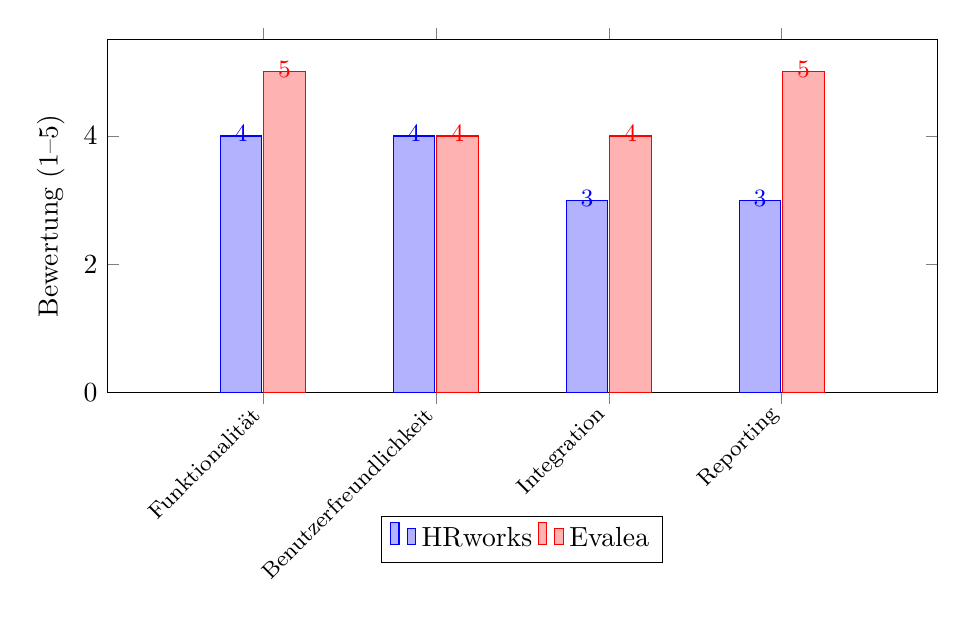
\begin{tikzpicture}
        \begin{axis}[
            width=\textwidth,
            height=0.5\textwidth,
            ybar=0.7pt,
            bar width=15pt,
            enlarge x limits=0.3,
            ylabel={Bewertung (1–5)},
            symbolic x coords={Funktionalität, Benutzerfreundlichkeit, Integration, Reporting},
            xtick=data,
            x tick label style={font=\footnotesize, rotate=45, anchor=east},
            ymin=0, ymax=5.5,
            nodes near coords,
            nodes near coords style={font=\small, anchor=mid},
            legend style={at={(0.5,-0.35)}, anchor=north, legend columns=-1},
            legend cell align={left}
        ]
        \addplot[blue,fill=blue!30] coordinates {
            (Funktionalität,4)
            (Benutzerfreundlichkeit,4)
            (Integration,3)
            (Reporting,3)
        };
        \addplot[red,fill=red!30] coordinates {
            (Funktionalität,5)
            (Benutzerfreundlichkeit,4)
            (Integration,4)
            (Reporting,5)
        };
        \legend{HRworks, Evalea}
        \end{axis}
    \end{tikzpicture}
    \caption{Visueller Vergleich zwischen HRworks und Evalea in verschiedenen Kategorien.}
    \label{fig:hrworks_evalea_comparison}
\end{figure}






\begin{figure}[h!]
    \centering
    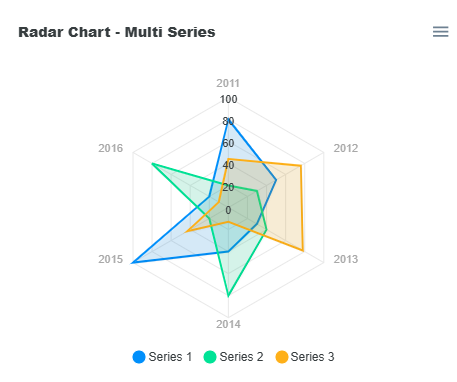
\includegraphics[width=0.8\textwidth]{images/radarchart_apexcharts.png}
    \caption{Framework Apexcharts für React}
    \label{fig:hrworks_evalea_comparison}
\end{figure}

Die Analyse zeigt, dass beide Tools ihre Stärken haben, jedoch keines vollständig die Anforderungen an spezialisierte Mitarbeitendengesprächs-Reporting-Tools erfüllt. Das geplante Tool zielt darauf ab, diese Lücken zu schließen.

	\chapter{Konzeption des Systems}
\label{chap:konzeption}

\section{\"Uberblick}
Die Konzeption des Systems bildet das Fundament für die spätere Implementierung und vereint moderne Technologien, um eine leistungsfähige und benutzerfreundliche Mitarbeitergesprächssoftware zu entwickeln. Im Zentrum der Konzeption stehen drei essenzielle Bereiche: das Design, die technischen Komponenten und die Datenarchitektur.

Das System zielt darauf ab, durch die Kombination von Frontend-Technologien wie React und Vite mit einem effizienten Backend auf Basis von .NET Core eine skalierbare und zuverlässige Plattform zu schaffen \cite{kirk2016data, microsoftDotNet}. Ergänzt wird dies durch eine relationale Datenbankstruktur, die mit Azure SQL realisiert wird, um eine robuste und sichere Speicherung sowie Verarbeitung der Gesprächsdaten zu gewährleisten \cite{azureDocumentation}.

Ein besonderer Fokus liegt auf der Interoperabilität mit bestehenden HR-Infrastrukturen. Durch den Einsatz von Microsoft Azure-Diensten wie Active Directory und Microsoft Graph wird eine nahtlose Integration ermöglicht, die nicht nur die Benutzerfreundlichkeit steigert, sondern auch die Effizienz datenbasierter Entscheidungsprozesse fördert \cite{microsoftAzure}. Die Architektur ist darauf ausgelegt, Visualisierungstools wie Donut- und Radarcharts zu integrieren, die eine intuitive und präzise Darstellung komplexer Daten unterstützen \cite{evergreen2016effective}.

Diese Konzeption stellt sicher, dass die verschiedenen Komponenten des Systems harmonisch zusammenwirken, um den Anforderungen moderner Arbeitsumgebungen gerecht zu werden und gleichzeitig die Grundlage für eine zukunftssichere Weiterentwicklung zu schaffen.


\section{Systemarchitektur}
Die Systemarchitektur basiert auf einem klassischen Client-Server-Modell, das eine klare Trennung zwischen der Benutzeroberfläche und den serverseitigen Prozessen gewährleistet. Diese Architektur erlaubt eine modulare und skalierbare Entwicklung, die sowohl Benutzerfreundlichkeit als auch Systemeffizienz priorisiert.

Das Frontend wird mit React entwickelt, einer modernen JavaScript-Bibliothek, die durch ihre komponentenbasierte Struktur eine effiziente Erstellung und Wiederverwendbarkeit von Benutzeroberflächen ermöglicht \cite{stefanov2021react}. Um die Entwicklungszeit zu verkürzen und eine optimale Performance zu gewährleisten, wird Vite als Build-Tool eingesetzt. Die visuelle Darstellung von Daten wird durch Bibliotheken wie ApexCharts unterstützt, die interaktive und ansprechende Diagramme ermöglichen \cite{apexchartsDoc}.

Das Backend wird mit .NET Core realisiert, einem plattformunabhängigen Framework, das sich durch hohe Performance und Flexibilität auszeichnet \cite{microsoftDotNet}. Es stellt RESTful APIs bereit, die die Kommunikation zwischen Frontend und Backend ermöglichen, und verwendet Azure-Dienste wie den Azure Service Bus für die Integration von asynchronen Prozessen \cite{azureServiceBus}. Azure Active Directory wird für die sichere Authentifizierung der Benutzer eingesetzt, während Azure SQL eine robuste Datenbanklösung für die Speicherung und Verarbeitung von Daten bereitstellt \cite{azureDocumentation}.

Durch die Kombination dieser Technologien wird sichergestellt, dass das System eine hohe Skalierbarkeit, Stabilität und nahtlose Integration in bestehende Infrastrukturen bietet. Diese modulare Architektur unterstützt eine schnelle Weiterentwicklung und Anpassung an zukünftige Anforderungen.


\subsection{Frontend-Architektur}

Das Frontend des Systems wird mit React und Vite entwickelt, um eine hohe Performance und schnelle Entwicklungszyklen zu gewährleisten. React dient als Kerntechnologie für die komponentenbasierte Architektur, während Vite als moderner Build-Toolchain für eine optimale Ladezeit und Hot-Module-Replacement verwendet wird.

\subsubsection*{Technische Grundlagen und Implementierung} 
Das Frontend nutzt TypeScript, um durch statische Typisierung die Lesbarkeit und Wartbarkeit des Codes zu erhöhen. Weiterhin werden die folgenden Technologien und Bibliotheken verwendet: 
\begin{itemize}
    \item \textbf{@azure/msal-browser und @azure/msal-react:} Zur sicheren Benutzer-Authentifizierung über Azure Active Directory und nahtlosen Integration in die Azure-Dienste.
    \item \textbf{@reduxjs/toolkit und Zustand:} Für ein effizientes State-Management, das die Synchronisierung von Benutzerinteraktionen und Daten sicherstellt.
    \item \textbf{Primereact und Fluent UI:} Für die Erstellung moderner und zugänglicher Benutzeroberflächen-Komponenten.
    \item \textbf{Axios:} Für die Kommunikation mit den RESTful-APIs des Backends.
    \item \textbf{Apexcharts und React-Apexcharts:} Zur Datenvisualisierung, insbesondere für Donut- und Radarcharts, die zur Darstellung von Mitarbeitendengesprächsdaten genutzt werden.
    \item \textbf{CSS-Module-Plugins:} Um die Modularität und Wiederverwendbarkeit von Stilen sicherzustellen.
\end{itemize}

\subsubsection*{Prototyping und Benutzerzentrierung} 
Für das Prototyping und die Abstimmung mit Stakeholdern wird Figma verwendet, um frühzeitig Feedback zur Benutzeroberfläche einzuholen und diese iterativ zu verbessern. Dieser Ansatz sichert eine benutzerzentrierte Entwicklung, die den Anforderungen der Zielgruppe entspricht.

\subsubsection*{Entwicklungsprozesse und DevOps} 
Das Projekt wird mittels Azure Pipelines in eine CI/CD-Pipeline integriert. Dies ermöglicht automatisierte Tests und Deployments des Frontends in verschiedene Umgebungen. Zudem wird Docker für die Containerisierung genutzt, um eine konsistente Entwicklungs- und Produktionsumgebung sicherzustellen.

\subsubsection*{Abstimmung von Komponenten und Workflows} 
Ein besonderer Fokus liegt auf der Entwicklung wiederverwendbarer UI-Komponenten, die für verschiedene Anwendungsfälle angepasst werden können. Hierzu zählen insbesondere: 
\begin{itemize}
    \item Visualisierungskomponenten wie Donut- und Radarcharts für die Datenanalyse.
    \item Formulare und Interaktionskomponenten, die eine intuitive Dateneingabe und Navigation ermöglichen.
    \item Dashboards, die eine zentrale Übersicht über die analysierten Daten bieten.
\end{itemize}

Durch den Einsatz dieser Technologien und Prinzipien bietet das Frontend eine hohe Benutzerfreundlichkeit, Performance und Skalierbarkeit, die den Anforderungen moderner HR-Tools gerecht wird.


\subsection{Backend-Architektur}

Das Backend des Systems wird mit .NET Core entwickelt, um eine robuste und skalierbare Grundlage für die Verarbeitung und Speicherung der Daten zu gewährleisten. Es umfasst mehrere zentrale Dienste und Technologien, die zusammen eine effiziente und sichere Systemarchitektur ermöglichen.\cite{azureArchitecture2024}

\subsubsection*{Zentrale Dienste und Technologien}
Das Backend basiert auf einer modularen Architektur und integriert die folgenden Komponenten:
\begin{itemize}
    \item \textbf{Azure Service Bus:} Wird für die Verarbeitung und Synchronisation von Nachrichten zwischen den verschiedenen Systemkomponenten eingesetzt. Diese Technologie ermöglicht die asynchrone Kommunikation und trägt zur Skalierbarkeit des Systems bei.\cite{azureServiceBus2024}
    \item \textbf{DBContext:} Entity Framework Core wird für den Datenbankzugriff verwendet, wodurch eine einfache Verwaltung und Abfrage der relationalen Datenbank ermöglicht wird.\cite{entityFrameworkCore2020}
    \item \textbf{Hintergrundjobs:} Automatisierte Aufgaben wie das Verarbeiten von Berichten, das Versenden von Benachrichtigungen oder das Berechnen aggregierter Daten werden über geplante Hintergrundprozesse realisiert.\cite{backgroundTasks2017}
    \item \textbf{RESTful APIs:} Das Backend stellt definierte Endpunkte für die Kommunikation mit dem Frontend bereit, um den sicheren und effizienten Austausch von Daten zu gewährleisten \cite{microsoftDotNet}.
\end{itemize}

\subsubsection*{Technologien und Abhängigkeiten}
Das Backend verwendet moderne Technologien und Bibliotheken, um die Anforderungen an Sicherheit, Performance und Skalierbarkeit zu erfüllen. Zu den zentralen Abhängigkeiten zählen:
\begin{itemize}
    \item \textbf{AutoMapper:} Für die Abbildung von Datenmodellen und DTOs (Data Transfer Objects), was die Wartbarkeit und Lesbarkeit des Codes verbessert.\cite{automapperDocs2024}.
    \item \textbf{MassTransit und MassTransit.Azure.ServiceBus.Core:} Diese Bibliotheken ermöglichen die Implementierung von Messaging-Lösungen und die Integration mit Azure Service Bus.\cite{masstransit2021}.
    \item \textbf{Microsoft.AspNetCore.Authentication.JwtBearer:} Für die Authentifizierung und Autorisierung von Benutzern mithilfe von JSON Web Tokens (JWT).\cite{jwtAuthDocs2024}.
    \item \textbf{Microsoft.EntityFrameworkCore:} Für die datenbankseitige Verarbeitung, einschließlich Unterstützung für SQL Server.\cite{efCoreDocs2024}.
    \item \textbf{Microsoft.AspNet.OData und Microsoft.AspNetCore.OData:} Zur Unterstützung von OData-Abfragen, die flexible Datenabfragen ermöglichen.\cite{odata2022}.
\end{itemize}

\subsection{Integration mit Microsoft Services}

Das Backend ist tief in die Microsoft Azure-Infrastruktur integriert, um maximale Effizienz und Sicherheit zu gewährleisten:
\begin{itemize}
    \item \textbf{Azure Active Directory (AAD):} Ermöglicht die sichere Authentifizierung der Benutzer und die Integration mit anderen Azure-Diensten.\cite{azureAD2021}.
    \item \textbf{Microsoft Graph API:} Unterstützt die Abfrage von Benutzer- und Organisationsdaten, um die Integration in bestehende HR-Systeme zu erleichtern.\cite{microsoftGraph2020}.
    \item \textbf{Azure Pipelines:} Wird für Continuous Integration und Continuous Deployment (CI/CD) verwendet, wodurch der Entwicklungs- und Bereitstellungsprozess automatisiert wird.\cite{azurePipelines2021}.
\end{itemize}

\subsection{Datenbankdesign}

Die Datenbank ist das Rückgrat des Systems und basiert auf einer relationalen Struktur, die mit Microsoft SQL Server realisiert wird. Die Haupttabellen umfassen:
\begin{itemize}
    \item \textbf{EmployeeAppraisalData:} Speichert Stammdaten der Mitarbeitenden, wie Namen, Jobtitel und IDs.
    \item \textbf{EmployeeAppraisal:} Enthält spezifische Daten zu Mitarbeitendengesprächen, wie Datum, beteiligte Personen und Ergebnisse.
    \item \textbf{AppraisalGroup, AppraisalSubgroup, AppraisalQuestion:} Diese Tabellen strukturieren die Inhalte und Fragen der Gespräche.
    \item \textbf{AppraisalStatus:} Dokumentiert den aktuellen Fortschritt eines Mitarbeitendengesprächs, z. B. „In Bearbeitung“ oder „Abgeschlossen“.
\end{itemize}

Die Struktur der Datenbank ist darauf ausgelegt, eine effiziente Speicherung und Verarbeitung großer Datenmengen zu ermöglichen. Zusätzlich wird die Datenbank über Entity Framework Core angebunden, um eine einfache Interaktion mit der Anwendungsschicht zu gewährleisten.

\subsubsection*{Sicherheitsmaßnahmen}
Die Datenbank ist vollständig verschlüsselt, und der Zugriff erfolgt ausschließlich über authentifizierte und autorisierte Kanäle. Rollenspezifische Zugriffsrechte stellen sicher, dass sensible Daten nur von berechtigten Benutzern eingesehen und bearbeitet werden können.
\cite{liu2021security}
\subsubsection*{Zusammenfassung}
Das Backend bildet die Grundlage für die datenbasierte Analyse und Visualisierung von Mitarbeitendengesprächsdaten. Durch die Integration moderner Technologien und Sicherheitsmechanismen stellt es eine performante, skalierbare und sichere Lösung für die Anforderungen des Systems dar.\cite{microsoft2020azure}


\subsection{Datenbankstruktur}
\begin{itemize}
    \item \textbf{EmployeeAppraisalData:} Speichert die Stammdaten der Mitarbeitenden, einschlie\ss lich Name, Microsoft-ID und Jobtitel.
    \item \textbf{EmployeeAppraisal:} Enth\"alt die Informationen zu den einzelnen Mitarbeitendengespr\"achen, wie das Datum und die beteiligten Personen.
    \item \textbf{AppraisalGroup, AppraisalSubgroup, AppraisalQuestion:} Diese Tabellen strukturieren die Fragen und Gruppierungen innerhalb eines Mitarbeitendengespr\"achs.
    \item \textbf{AppraisalStatus:} Verfolgt den Status eines Gespr\"achs, z. B. \glqq In Bearbeitung\grqq{} oder \glqq Abgeschlossen\grqq{}.
\end{itemize}

\begin{table}[h!]
\centering
\caption{Zusammenfassung der wichtigsten Datenbanktabellen}
\label{tab:db_overview}
\begin{tabularx}{\textwidth}{|X|X|}
\hline
\textbf{Tabelle} & \textbf{Beschreibung} \\\hline
EmployeeAppraisalData & Speichert Stammdaten der Mitarbeitenden. \\\hline
EmployeeAppraisal & Enth\"alt Informationen zu Mitarbeitendengespr\"achen. \\\hline
AppraisalGroup & Gruppiert verschiedene Fragen innerhalb eines Gespr\"achs. \\\hline
AppraisalSubgroup & Unterteilt die Gruppen in spezifischere Themenbereiche. \\\hline
AppraisalQuestion & Speichert die Fragen eines Gespr\"achs. \\\hline
AppraisalStatus & Dokumentiert den aktuellen Status eines Gespr\"achs. \\\hline
\end{tabularx}
\end{table}

\subsection{Beziehungsmodell}
Die Datenbank ist relational aufgebaut, um eine effiziente Speicherung und Abfrage von Daten zu gew\"ahrleisten. Abbildung \ref{fig:db_er_model} zeigt das ER-Diagramm des Systems.

\begin{figure}[h!]
    \centering
    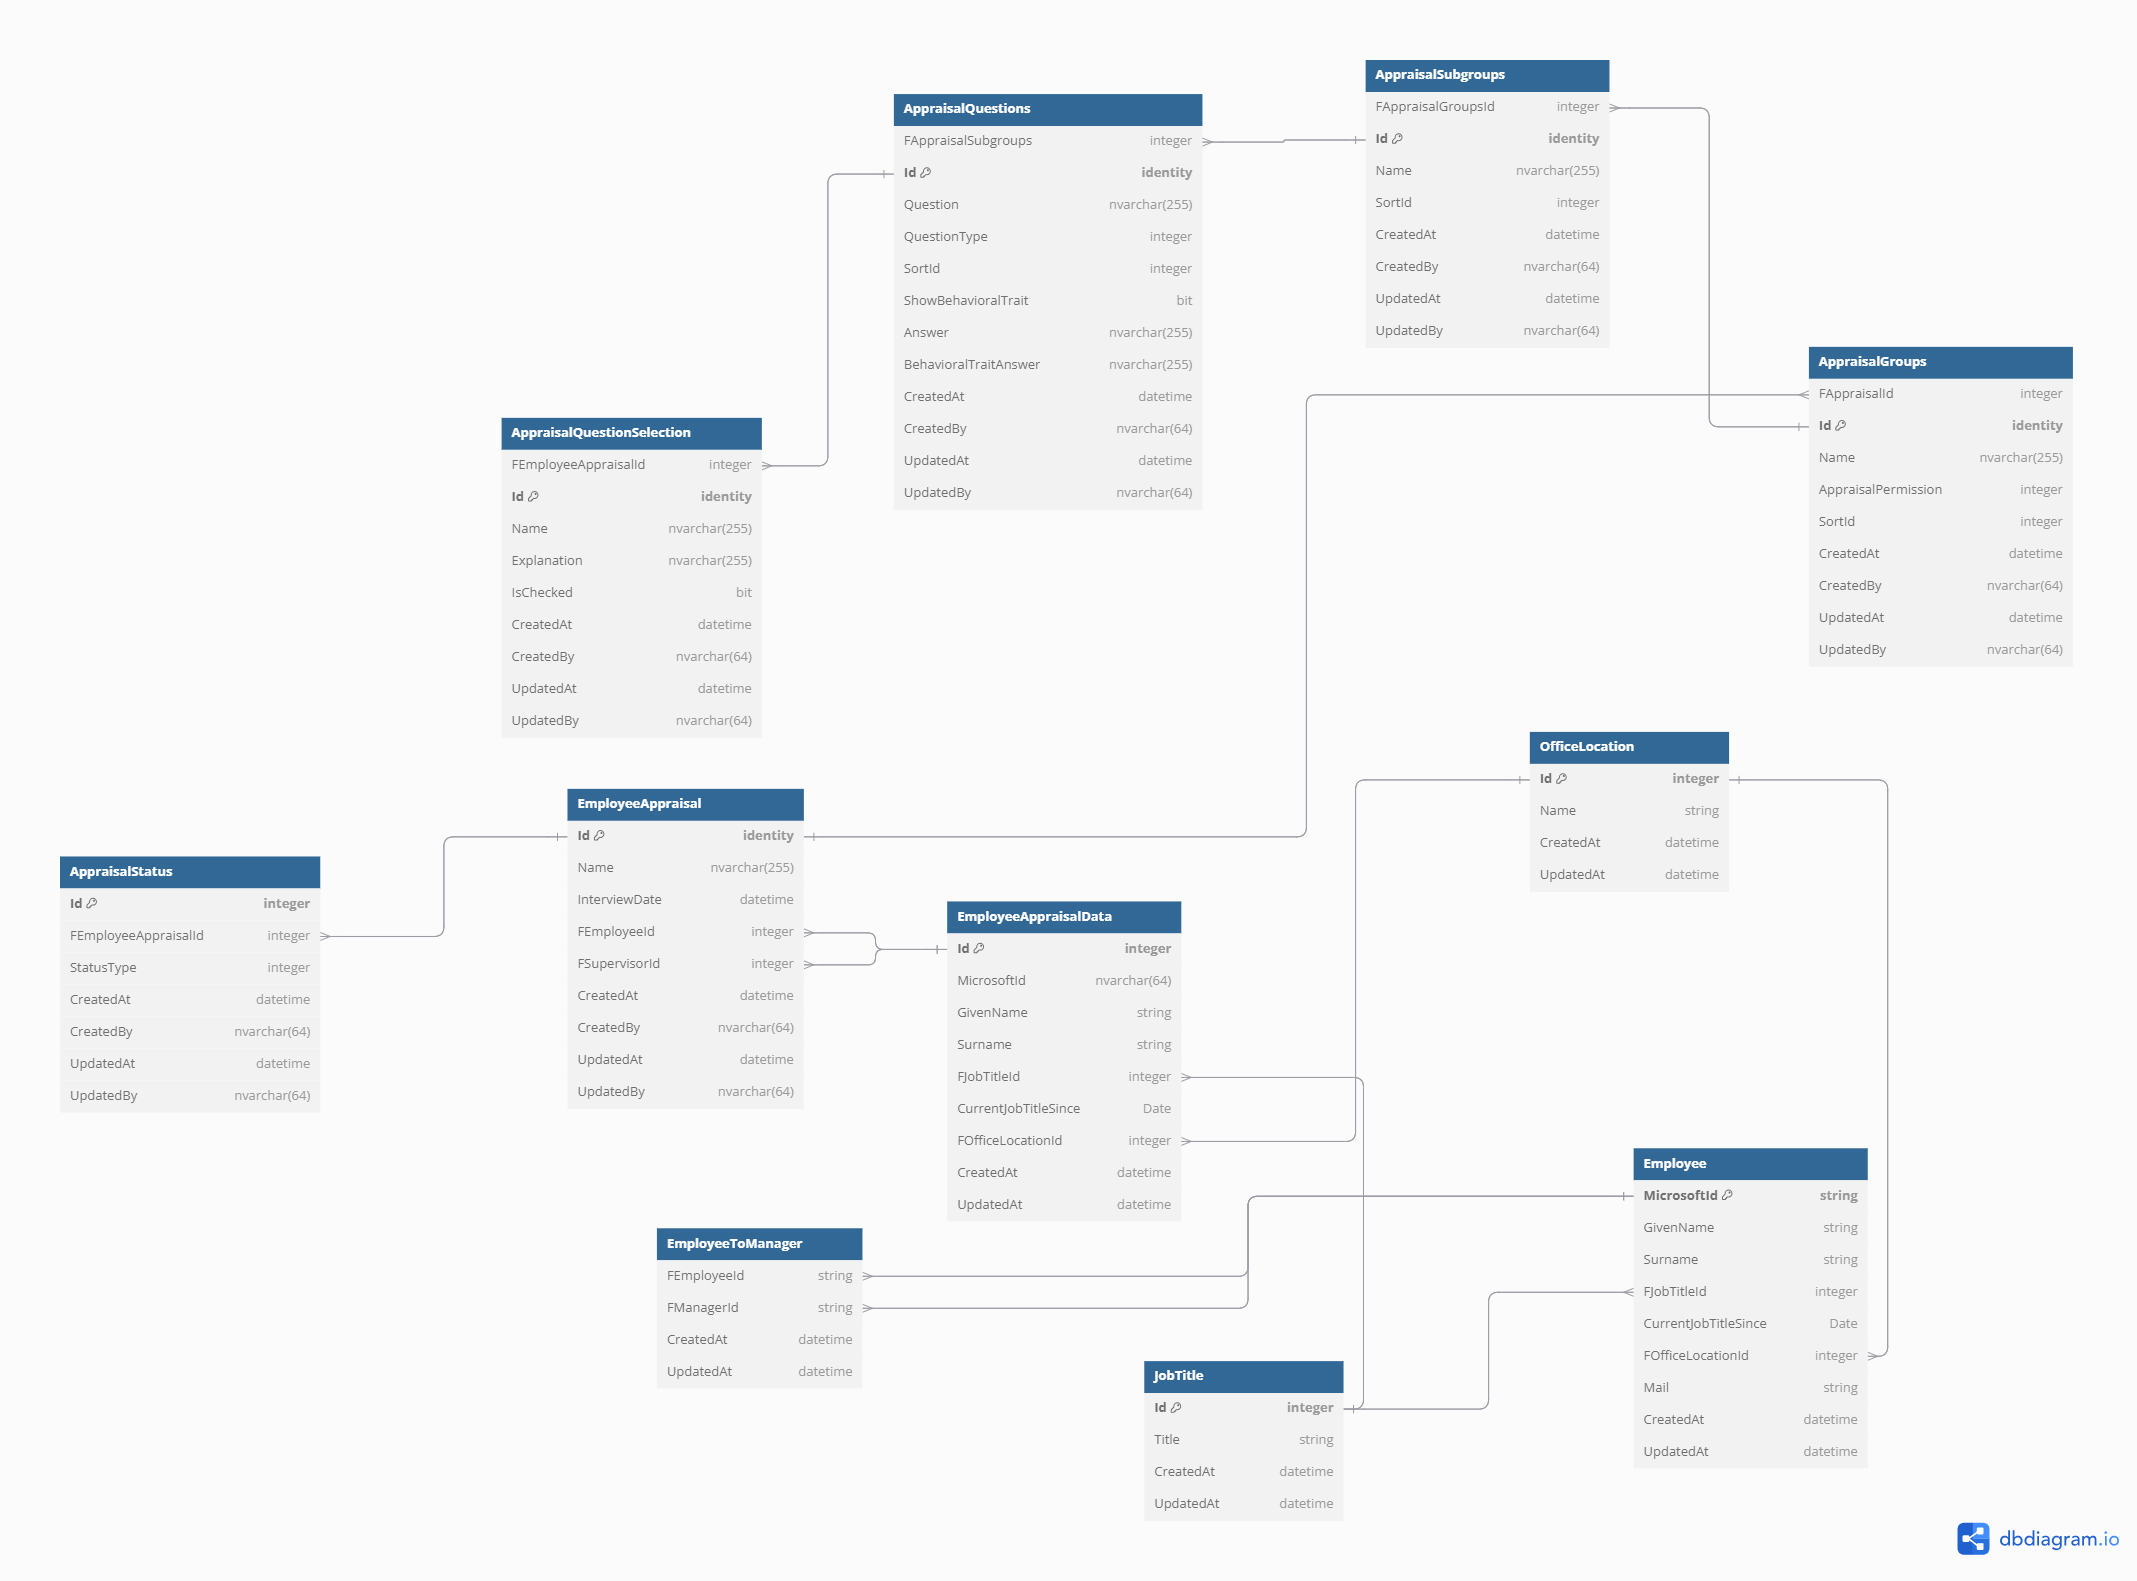
\includegraphics[width=0.8\textwidth]{images/er_modell_design.png}
    \caption{ER-Diagramm der Datenbankstruktur.}
    \label{fig:db_er_model}
\end{figure}

\section{Workflows}
Die Konzeption des Systems umfasst klar definierte Workflows, um eine reibungslose Funktionalität und Effizienz sicherzustellen:
\begin{itemize}
    \item \textbf{Datenimport:} Mitarbeitendengesprächsdaten werden über das Backend in die relationale Datenbank importiert. Hierbei wird eine automatische Validierung der Eingabedaten durchgeführt, um die Datenqualität sicherzustellen \cite{gupta2020data, prat2021pipeline}.
    \item \textbf{Datenverarbeitung:} Geplante Hintergrundjobs übernehmen Aufgaben wie die Berechnung aggregierter Statistiken, das Generieren von Berichten oder das Versenden von Benachrichtigungen an berechtigte Benutzer \cite{hollingsworth2020workflow, apache2023workflow}.
    \item \textbf{Visualisierung:} Die aufbereiteten Daten werden über definierte RESTful APIs an das Frontend übermittelt, wo sie durch interaktive Diagramme wie Donut- und Radarcharts anschaulich dargestellt werden \cite{kirk2016data, evergreen2016effective}.
\end{itemize}


\section{Sicherheitskonzepte}
Die Sicherheit des Systems wird durch mehrere bewährte Maßnahmen gewährleistet, um Datenintegrität und Vertraulichkeit sicherzustellen:
\begin{itemize}
    \item \textbf{Authentifizierung:} Benutzer authentifizieren sich über Azure Active Directory (AAD), das Multi-Faktor-Authentifizierung (MFA) und Single Sign-On (SSO) unterstützt \cite{microsoftAAD}.
    \item \textbf{Datenverschlüsselung:} Alle sensiblen Daten, sowohl im Ruhezustand als auch während der Übertragung, werden durch moderne Verschlüsselungsmethoden wie AES-256 geschützt \cite{schneier2015applied}.
    \item \textbf{Rechteverwaltung:} Eine fein granulierte, rollenspezifische Zugriffskontrolle (RBAC) stellt sicher, dass nur autorisierte Benutzer auf spezifische Daten und Funktionen zugreifen können \cite{ferraiolo2003rbac}.
\end{itemize}


\section{Zusammenfassung}
Die vorgestellte Konzeption kombiniert innovative Technologien, effiziente Workflows und umfassende Sicherheitsmaßnahmen, um eine performante und skalierbare Lösung für die Verwaltung und Visualisierung von Mitarbeitendengesprächsdaten zu gewährleisten. Durch den gezielten Einsatz moderner Entwicklungs- und Sicherheitsstandards wird eine benutzerfreundliche und zuverlässige Plattform geschaffen, die den Anforderungen sowohl auf technischer als auch auf organisatorischer Ebene gerecht wird.


	\chapter{Implementierung}
\label{chap:implementierung}

\section{Technologische Basis}
Die Implementierung basiert auf einer sorgfältig ausgewählten technologischen Basis, die modernste Tools und Frameworks kombiniert, um eine effiziente, skalierbare und sichere Lösung zu gewährleisten. Die Haupttechnologien umfassen:

Für das Frontend wurde React und TypeScript verwendet, um eine robuste und komponentenbasierte Architektur zu gewährleisten. Primereact wird als (\hyperref[abkuerzungen]{UI})-Bibliothek eingesetzt, um eine konsistente Benutzeroberfläche zu realisieren und die Entwicklungszeit durch vorgefertigte, anpassbare Komponenten zu verkürzen \cite{facebook2021react}. Vite dient als modernes Build-Tool, das durch schnelle (\hyperref[abkuerzungen]{HMR})-Funktionen eine produktive Entwicklungsumgebung bietet \cite{vite2022docs}.

Im Backend wird.NET Core als Technologie benutzt, um RESTful (\hyperref[abkuerzungen]{APIs}) bereitzustellen, die eine zuverlässige und standardisierte Kommunikation ermöglichen \cite{fielding2000rest}. Middleware-Services wurden implementiert, um Aufgaben wie Authentifizierung, Fehlerbehandlung und Protokollierung zu übernehmen. Die Verwendung von (\hyperref[abkuerzungen]{AAD}) gewährleistet eine sichere Authentifizierung und rollenbasierte Zugriffskontrolle \cite{aad2023}.

Die Azure Cloud spielt eine zentrale Rolle bei der Implementierung, da sie Dienste wie Azure Service Bus zur asynchronen Kommunikation zwischen Anwendungen bereitstellt \cite{azureServiceBus2024}. Außerdem ermöglicht sie eine flexible und skalierbare Infrastruktur, die für die Anforderungen des Systems optimiert ist \cite{azureDocumentation}.

Zur Optimierung des Entwicklungs- und Bereitstellungsprozesses werden automatisierte CI/CD-Pipelines mit 
Azure Pipelines verwendet. Diese Pipelines integrieren automatisierte Tests, Builds und Deployments, um eine hohe Qualität und schnelle Iterationen sicherzustellen \cite{ciCdScalability}.
Die Entwicklung wurde mit der Versionsverwaltungtool Git begleitet. Es ermöglicht effizientes Arbeiten mit Feature-Branches, Pull-Requests und das einfache Nachverfolgen von Änderungen. GitHub wurde als zentrale Plattform für die Zusammenarbeit und Code-Reviews verwendet \cite{chacon2021git}.

Im Azure (\hyperref[abkuerzungen]{DevOps}) wurde ein digitales SCRUM-Board  eingesetzt. Es dient dazu Aufgaben/Features zu aufzunehmen und priorisieren und den Fortschritt in Sprints zu überwachen \cite{scrumGuide}.

Um die einzelnen Komponenten zu testen wurde die Tools wie Jest und React Testing Library wurden zur Sicherstellung der Codequalität eingesetzt \cite{jestDocumentation}. 
Automatisierte Tests wurden in die (\hyperref[abkuerzungen]{CI/CD})-Pipeline integriert, um frühzeitig Fehler zu erkennen und zu beheben.
Für die Bereitstellung einer konsistenten Entwicklungs- und Produktionsumgebung wurde Docker genutzt. Docker-Images für das Frontend und Backend werden in einer Azure Container Registry (\hyperref[abkuerzungen]{ACR}) gespeichert und ermöglichen schnelle und skalierbare Deployments \cite{dockerScalability}.

Zum Monitoring und Fehleranalyse wurde Azure Application Insights zur Überwachung von Systemmetriken wie Antwortzeiten, Fehlerraten und Benutzerinteraktionen integriert. Dies ermöglicht eine effiziente Fehlerdiagnose und Performance-Optimierung \cite{microsoftAppInsights}.


Diese technologische Basis bildet die Grundlage für die Implementierung einer modernen, leistungsfähigen Softwarelösung, die den Anforderungen an Skalierbarkeit, Sicherheit und Benutzerfreundlichkeit gerecht wird.


\section{Detailierte Architektur}
\subsection{Frontend-Architektur}
Das Frontend wurde mit einer komponentenbasierten Architektur entwickelt, die eine modulare und wiederverwendbare Struktur ermöglicht. Jedes (\hyperref[abkuerzungen]{UI})-Element wurde als eigenständige Komponente konzipiert, um sowohl die Wartbarkeit als auch die Wiederverwendbarkeit zu maximieren. Diese Architektur fördert eine klare Trennung der Verantwortlichkeiten und ermöglicht eine einfache Anpassung und Erweiterung der Benutzeroberfläche.

Die Projektstruktur, wie in Abbildung~\ref{fig:frontend_code_paradigm} dargestellt, folgt bewährten Best Practices der modernen Frontend-Entwicklung. Der Ordner \texttt{components} enthält alle UI-Komponenten, während der Ordner \texttt{store} die State-Management-Logik beherbergt. Globale Konfigurationen werden im Ordner \texttt{config} verwaltet, während allgemeine Funktionen und Hilfsprogramme im Ordner \texttt{utils} zentralisiert sind. Diese Struktur fördert die Lesbarkeit und Wartbarkeit des Codes und erleichtert die Zusammenarbeit in Teams \cite{reactDocumentation}.

\begin{figure}[h!] \centering 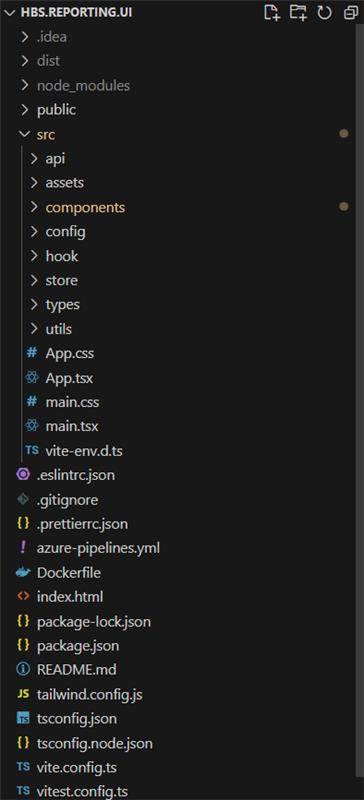
\includegraphics[width=0.4\textwidth]{images/frontendparadigma.jpg} \caption{Projektstruktur des Frontend-Paradigmas.} \label{fig:frontend_code_paradigm} \end{figure}

Ein weiteres zentrales Element ist das State-Management, das mithilfe von Redux Toolkit und Zustand realisiert wird. Redux Toolkit wurde für komplexe und globale Zustände gewählt, während Zustand für isolierte und lokale Zustände eingesetzt wird. Diese Kombination gewährleistet eine effiziente Verwaltung komplexer Datenflüsse innerhalb der Anwendung \cite{reduxToolkit}.

Darüber hinaus wurde ApexCharts in Kombination mit React-ApexCharts integriert, um interaktive Visualisierungen wie Donut- und Radarcharts zu erstellen. Diese Diagrammtypen sind essenziell für die Analyse und Darstellung von Mitarbeitendengesprächsdaten. Sie ermöglichen es den Benutzern, Trends und Muster intuitiv zu erkennen und fundierte Entscheidungen zu treffen \cite{apexchartsDoc}.

Zusammenfassend bietet die Frontend-Architektur eine flexible, skalierbare und benutzerfreundliche Basis, die die spezifischen Anforderungen des Projekts erfüllt. Sie gewährleistet nicht nur eine hohe Effizienz in der Entwicklung, sondern auch eine optimale Benutzererfahrung.

\begin{figure}[H]
    \centering
    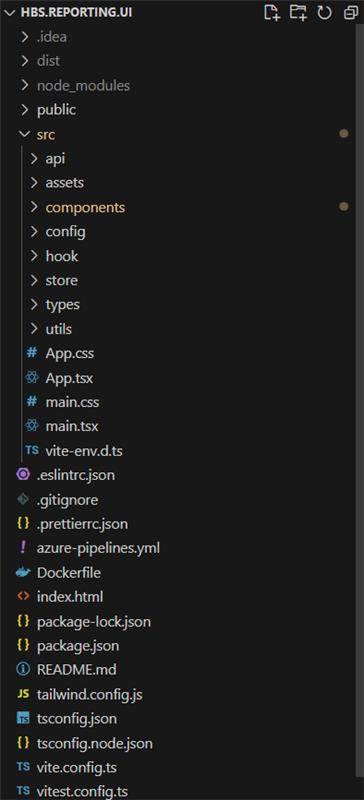
\includegraphics[width=0.4\textwidth, keepaspectratio]{images/frontendparadigma.jpg}
    \caption{Projektstruktur des Frontend-Paradigmas.}
    \label{fig:frontend_code_paradigm}
\end{figure}

In Abbildung~\ref{fig:frontend_code_paradigm} wird die Projektstruktur der Anwendung dargestellt. Die klare Trennung in Module wie \texttt{components}, \texttt{store} und \texttt{api} erleichtert nicht nur die Entwicklung, sondern fördert auch die Zusammenarbeit in Teams und die Skalierbarkeit des Systems. Diese Struktur bietet eine solide Grundlage für die Entwicklung moderner und leistungsstarker Webanwendungen.


\subsubsection*{Live Anwendung}
Die folgenden Abbildungen zeigen die (\hyperref[abkuerzungen]{PROD})-Ausschnitte der Anwendung:


\begin{figure}[H] \centering 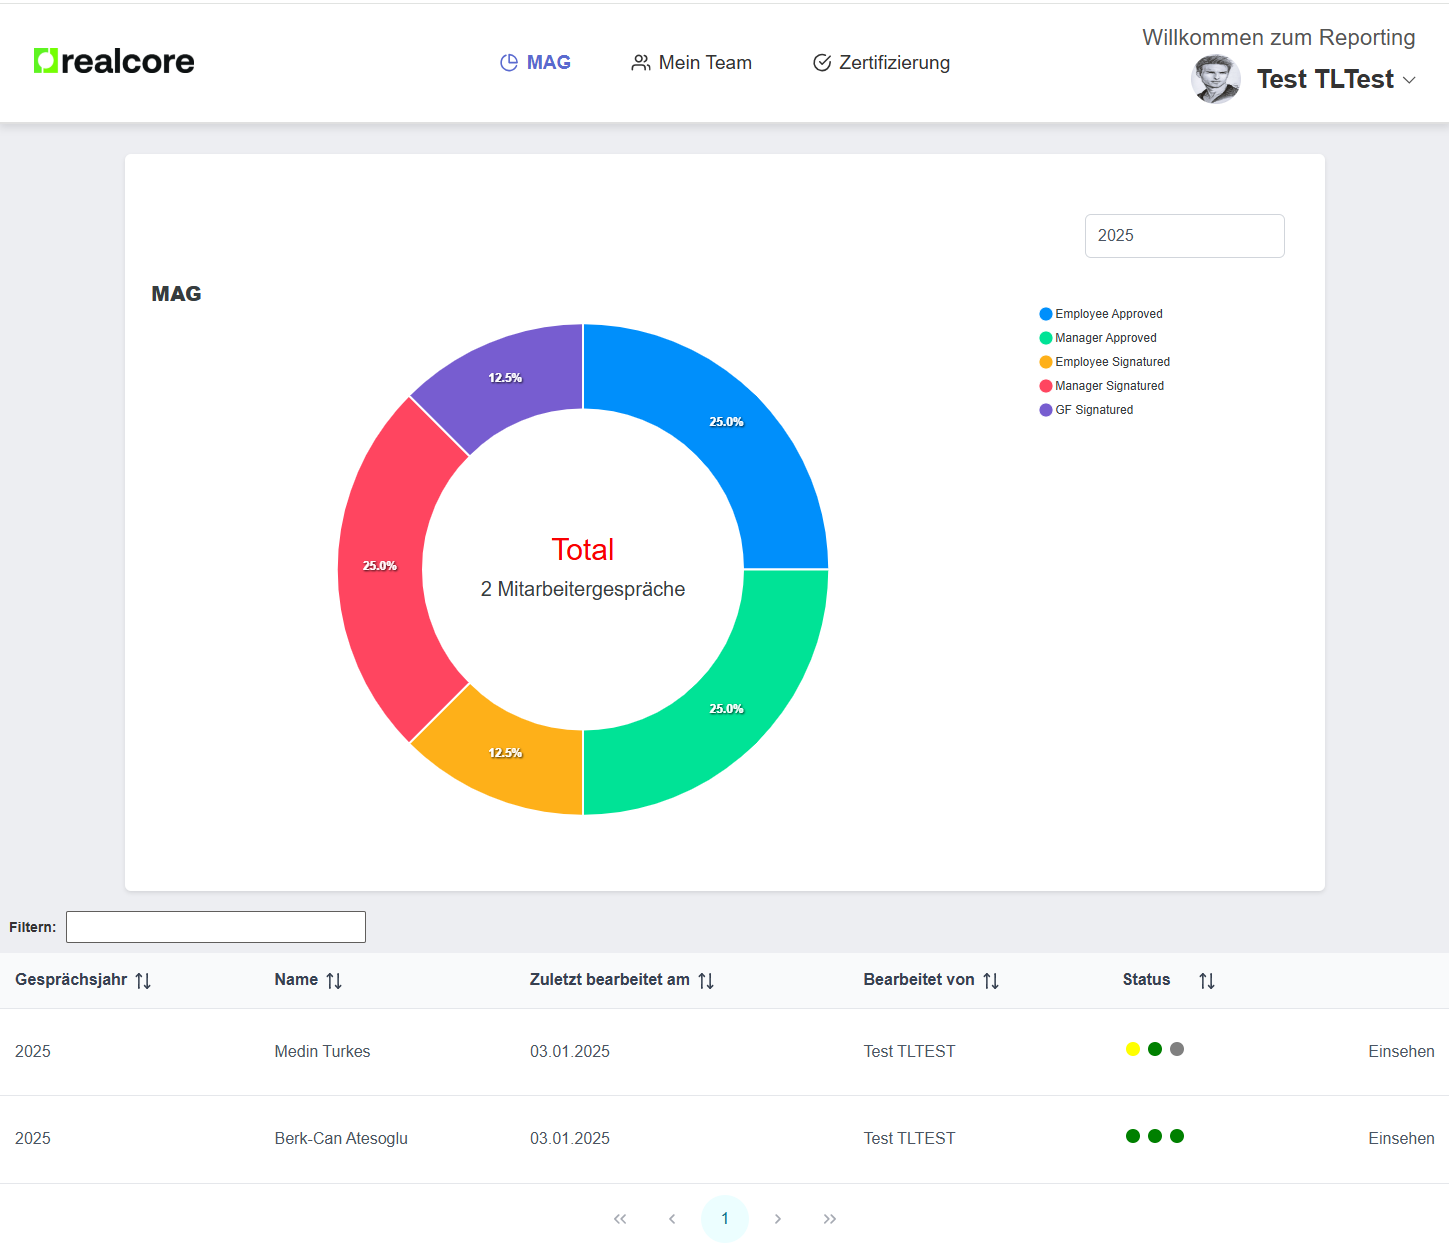
\includegraphics[width=\textwidth]{images/donutchart.png} \caption{Dashboard der Anwendung mit Donutchart und Übersicht über alle Mitarbeitendengespräche.} \label{fig:dashboard} \end{figure}

\begin{figure}[H] \centering 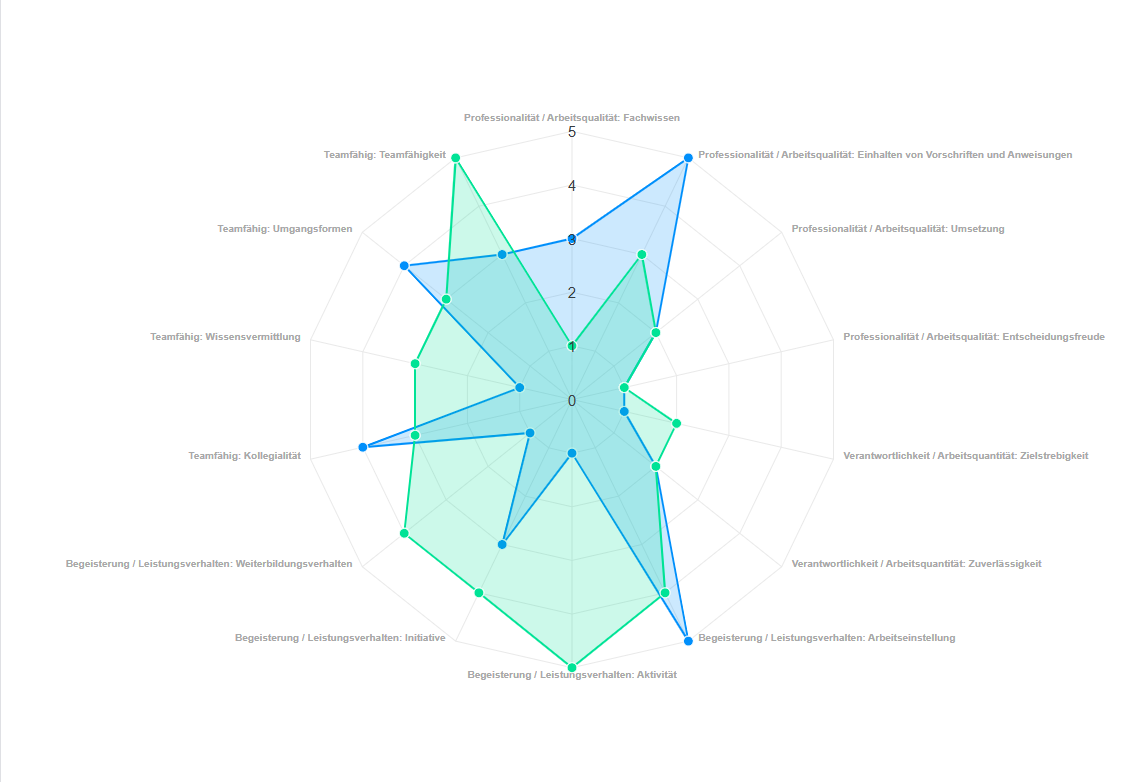
\includegraphics[angle=90, width=\textwidth]{images/radarchart_prod.png} \caption{Radarchart-Visualisierung der 1-5 Single Choice Antworten der Mitarbeitendengesprächsdaten.} \label{fig:radar_chart} \end{figure}

\begin{figure}[H] \centering 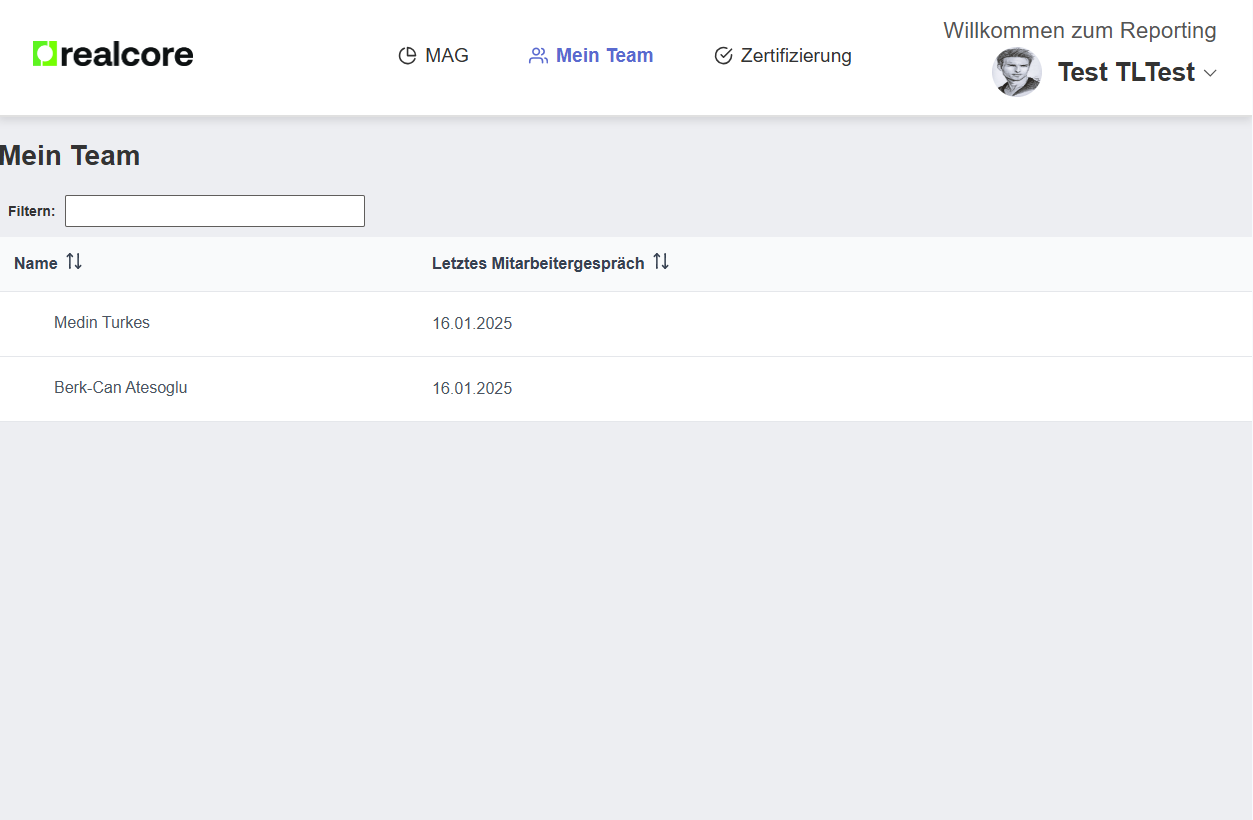
\includegraphics[width=\textwidth]{images/meinteam.png} \caption{Mein Team - Anzeige der Teammitglieder.} \label{fig:data_entry} \end{figure}

\begin{figure}[H]
    \centering
    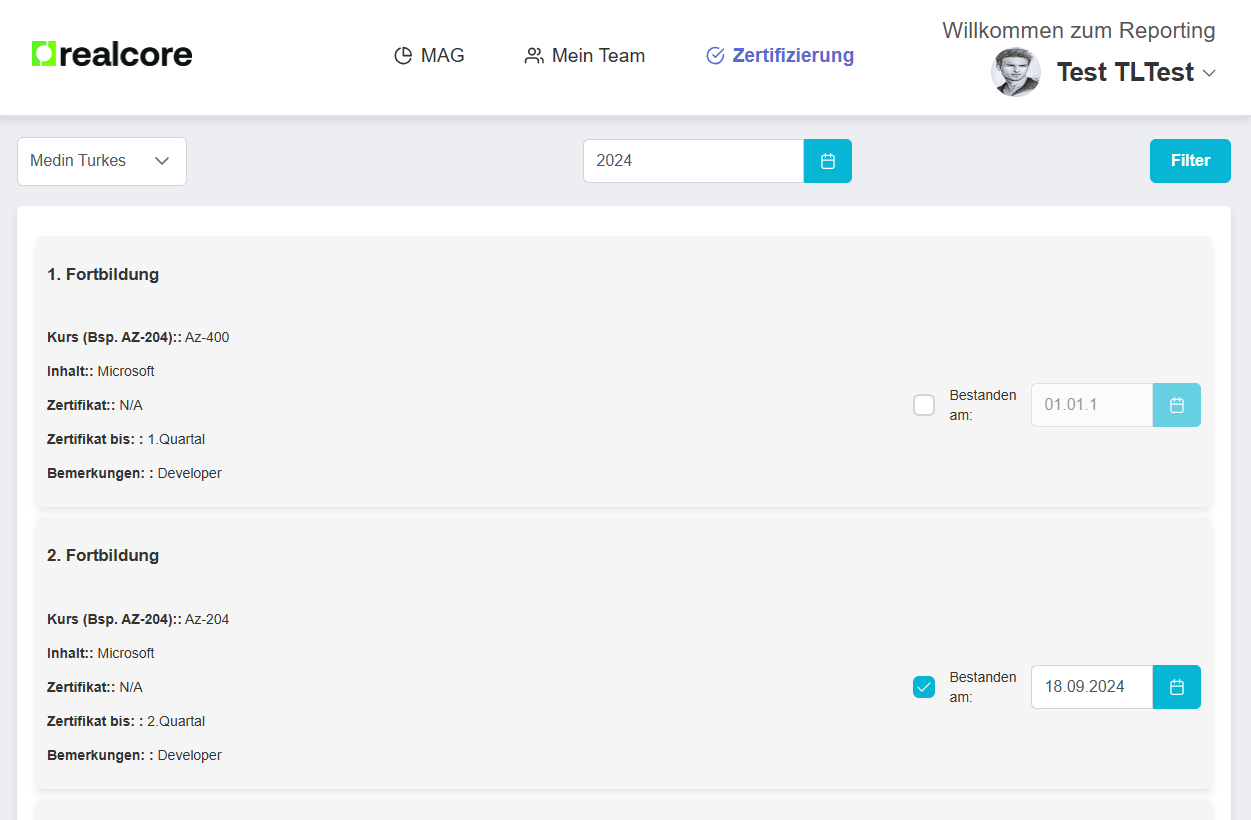
\includegraphics[width=\textwidth]{images/zertifkatshow.png}
    \caption{Anzeige der Mitarbeiterzertifizierungen mit der Möglichkeit, das Datum des bestandenen Zertifikats einzutragen.}
    \label{fig:zertifikatanzeige}
\end{figure}


\subsubsection*{Dockerfile für das Frontend}
Die Umsetzung des Frontends wurde durch die Nutzung von Docker als Containerisierungsplattform unterstützt, um eine konsistente Entwicklungs- und Produktionsumgebung zu gewährleisten. Das im Projekt verwendete Dockerfile basiert auf einem Multi-Stage-Build-Ansatz, der die Effizienz und Sicherheit der Anwendung optimiert. Im ersten Schritt wird die Anwendung mit Node.js gebaut, während im zweiten Schritt ein NGINX-Server verwendet wird, um die optimierten Dateien auszuliefern. Dieser Ansatz minimiert die Größe des finalen Containers und verbessert die Performance der Anwendung \cite{docker2020mastery, docker2019production}.

\begin{listing}[H]
\begin{minted}[linenos, frame=single, fontsize=\small]{dockerfile}
# Stage 0: Build the application
FROM node:16 as build-stage

WORKDIR /app

COPY package*.json /app/
RUN npm install --force

COPY vite.config.ts /app/
COPY vitest.config.ts /app/
COPY . /app/

RUN npm run build

# Stage 1: Serve the application using NGINX
FROM nginx:1.21
COPY --from=build-stage /app/dist/ /usr/share/nginx/html
\end{minted}
\caption{Dockerfile zur Containerisierung des Frontends}
\label{lst:dockerfile_frontend}
\end{listing}

In der ersten Build-Stage wird das Node.js-Image genutzt, das von der offiziellen Node.js-Docker-Bibliothek bereitgestellt wird \cite{node2021docker}. Hier werden die notwendigen Abhängigkeiten installiert und der Build-Prozess der Anwendung durchgeführt. Die zweite Stage verwendet ein NGINX-Image, das speziell für den Einsatz als Webserver optimiert ist \cite{nginx2021docker}. Der Multi-Stage-Ansatz bietet den Vorteil, dass lediglich die notwendigen Dateien für den Betrieb in die zweite Stage übernommen werden, wodurch die Größe des finalen Containers reduziert wird \cite{docker2020mastery}.

Die Wahl von Docker und Multi-Stage-Builds basiert auf der hohen Flexibilität und Effizienz dieser Technologie. Im Vergleich zu herkömmlichen Deployment-Ansätzen bietet Docker eine standardisierte Umgebung, die Fehler durch abweichende Konfigurationen zwischen Entwicklungs- und Produktionssystemen minimiert \cite{docker2019production}. Durch die Verwendung von offiziellen Docker-Images für Node.js und NGINX wird zudem sichergestellt, dass aktuelle Sicherheitsstandards eingehalten werden \cite{node2021docker, nginx2021docker}.



\subsection{Backend-Architektur}
Die Projektstruktur, wie in Abbildung~\ref{fig:backend_code_paradigm} dargestellt, basiert auf modernen Softwareentwicklungsprinzipien und wurde so gestaltet, dass eine klare Trennung der Verantwortlichkeiten gewährleistet ist. Dies trägt erheblich zur Wartbarkeit und Skalierbarkeit der Anwendung bei.

Die zentrale Logik für die Verarbeitung von (\hyperref[abkuerzungen]{HTTP})-Anfragen ist in der Controller-Schicht implementiert. Diese Schicht fungiert als Schnittstelle zwischen dem Frontend und den Backend-Diensten. Sie übernimmt das Routing von Anfragen, orchestriert die Kommunikation mit den anderen Schichten und sorgt für die konsistente Bearbeitung der Daten. Die Geschäftslogik ist in der Handler-Schicht ausgelagert. Diese Struktur entlastet die Controller von komplexen Prozessen und fördert die Modularität. Ein Handler führt notwendige Berechnungen, Validierungen oder Orchestrierungen durch, bevor die Ergebnisse zurück an den Controller gegeben werden \cite{fowler2002patterns}.

Die Datenzugriffsschicht ist im Repository-Ordner organisiert. Hier werden CRUD-Operationen (Create,Read,Update,Delete) mithilfe von (\hyperref[abkuerzungen]{EF Core}) realisiert. Diese Abstraktionsebene sorgt für einen konsistenten und wartbaren Zugriff auf die Datenbank. Die Datenstrukturen, die innerhalb des Systems verwendet werden, sind im Ordner \texttt{Models} definiert. Diese Modelle dienen als Bindeglied zwischen den einzelnen Schichten und sichern die Konsistenz der Daten. Ergänzend dazu werden im \texttt{Helper}-Ordner wiederverwendbare Funktionen und Werkzeuge zentralisiert, wie beispielsweise Logging- oder Utility-Funktionen \cite{efCoreDocs2023}.

Ein weiteres wichtiges Element ist der \texttt{Consumer}-Ordner, der die Logik zur Verarbeitung von Nachrichten aus asynchronen Kommunikationssystemen wie dem Azure Service Bus enthält. Diese Struktur ermöglicht die Umsetzung eines Publish-Subscribe-Musters, das die Skalierbarkeit und Entkopplung von Systemkomponenten sicherstellt \cite{azureServiceBus2024}.

Die Konfigurationen des Systems werden in der Datei \texttt{appsettings.json} verwaltet. Hier sind Verbindungszeichenfolgen zur Datenbank, (\hyperref[abkuerzungen]{API})-Schlüssel und andere Umgebungsvariablen hinterlegt. Diese zentrale Verwaltung ermöglicht eine einfache Anpassung der Anwendung an verschiedene Umgebungen, beispielsweise Entwicklung, Test oder Produktion \cite{microsoftCloudDesignPatterns}.

Abbildung~\ref{fig:backend_code_paradigm} veranschaulicht diese Projektstruktur. Sie zeigt die logische Organisation der Dateien und Ordner und verdeutlicht, wie die Trennung der Verantwortlichkeiten die Zusammenarbeit im Team sowie die Skalierbarkeit und Wartbarkeit der Anwendung erleichtert.

\begin{figure}[H]
    \centering
    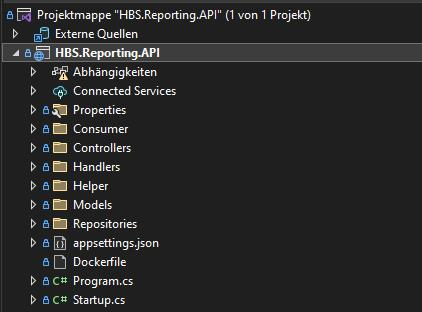
\includegraphics[width=0.8\textwidth, keepaspectratio]{images/backendparadigma.jpg}
    \caption{Projektstruktur des Backend-Paradigmas.}
    \label{fig:backend_code_paradigm}
\end{figure}

Diese strukturierte Herangehensweise bietet eine solide Grundlage für die Implementierung eines leistungsfähigen Backends. Durch die klare Trennung der Verantwortlichkeiten und die Verwendung bewährter Designprinzipien wird eine effiziente, skalierbare und wartungsfreundliche Architektur gewährleistet \cite{microsoftDotNetArchitecture}.




\subsection{Komponenten der Backend-Architektur}
Die Backend-Architektur folgt einer schichtbasierten Struktur, die eine klare Trennung von Verantwortlichkeiten ermöglicht. Diese modulare Architektur erleichtert die Wartbarkeit, Skalierbarkeit und Testbarkeit des Systems. Die Hauptkomponenten sind:

\begin{itemize}
     \item \textbf{Controller-Schicht:} Diese Schicht verarbeitet (\hyperref[abkuerzungen]{HTTP})-Anfragen und leitet sie an entsprechende Services weiter. Alternativen wie GraphQL wurden geprüft, aber aufgrund der Einfachheit und Standardisierung fiel die Wahl auf RESTful (\hyperref[abkuerzungen]{APIs}) \cite{fielding2000rest}.
\newpage
\begin{minted}[frame=single, fontsize=\small, linenos]{csharp}
using Microsoft.AspNetCore.Mvc;
using System.Threading.Tasks;

namespace HBS.Reporting.API.Controllers
{
    [ApiController]
    [Route("api/[controller]")]
    public class EmployeeAppraisalController : ControllerBase
    {
        private readonly IEmployeeAppraisalService _service;
        public 
        EmployeeAppraisalController(IEmployeeAppraisalService 
        service)
        {
            _service = service;
        }
        // GET: api/EmployeeAppraisal
        [HttpGet]
        public async Task<IActionResult> GetAll()
        {
            var appraisals = await _service.GetAllAppraisalsAsync();
            return Ok(appraisals);
        }
        // GET: api/EmployeeAppraisal/{id}
        [HttpGet("{id}")]
        public async Task<IActionResult> GetById(int id)
        {
            var appraisal = await _service.GetAppraisalByIdAsync(id);
            if (appraisal == null)
                return NotFound();
            return Ok(appraisal);
        }
        [HttpPost]
        public async Task<IActionResult> Create([FromBody] 
        EmployeeAppraisalDto dto)
        {
            if (!ModelState.IsValid)
                return BadRequest(ModelState);

            var createdAppraisal = await 
            _service.CreateAppraisalAsync(dto);
            return CreatedAtAction(nameof(GetById), 
            new { id = createdAppraisal.Id }, createdAppraisal);
        }
        [HttpDelete("{id}")]
        public async Task<IActionResult> Delete(int id)
        {
            var isDeleted = await _service.DeleteAppraisalAsync(id);
            if (!isDeleted)
                return NotFound();
            return NoContent();
        }
    }
}
\end{minted}

Dieser Code stellt einen Beispiel-Controller für die Verwaltung von Mitarbeitendengesprächen bereit. Die \texttt{GetAll}-Methode ruft alle vorhandenen Datensätze ab, während \texttt{GetById} spezifische Einträge anzeigt. Mit \texttt{Create} können neue Einträge erstellt und über \texttt{Delete} wieder gelöscht werden. Alle Anfragen werden an die Service-Schicht delegiert, was die Trennung von Logik und Schnittstellen gewährleistet.

    \item \textbf{Service-Schicht:} Diese Schicht implementiert die Geschäftslogik und orchestriert zwischen Controllern und Repositories. Alternativansätze, wie eine direkte Einbindung der Logik in die Controller, wurden verworfen, da sie die Wartbarkeit reduzieren würden.
    \item \textbf{Repository-Schicht:} Diese Schicht abstrahiert die Datenbankzugriffe mithilfe von Entity Framework Core und sorgt für konsistente Operationen \cite{efCoreDocs2023}.
    \item \textbf{Middleware:} Hier werden zentrale Funktionen wie Authentifizierung und Fehlerbehandlung implementiert, was die Controllerschicht entlastet.
\end{itemize}

\subsection{API-Endpunkte}
Zur Interaktion mit den Daten des Systems wurden verschiedene API-Endpunkte implementiert. Tabelle \ref{table:http-methods} listet die wesentlichen HTTP-Methoden und URLs zur Manipulation von Ressourcen auf:

\begin{table}[H]
\caption{(\hyperref[abkuerzungen]{HTTP})-Methoden und (\hyperref[abkuerzungen]{URLs}) zur Manipulation von Ressourcen}
\label{table:http-methods}
\raggedright
{\scriptsize Quelle: Eigene Darstellung} \\[0.3em]
\renewcommand{\arraystretch}{1.1}
\setlength{\tabcolsep}{1.8pt}
\begin{tabularx}{\textwidth}{>{\centering\arraybackslash}m{2cm}|>{\centering\arraybackslash}m{5.5cm}|>{\raggedright\arraybackslash}m{6.5cm}}
\hline
\textbf{HTTP-Methoden} & \textbf{URL /odata/v\{version\}} & \textbf{Beschreibung} \\\hline
GET & /employeeAppraisals/\{appraisalId\} & Lese ein einzelnes Mitarbeitenden- \linebreak gespräch anhand der eindeutigen ID. \\\hline
GET & /employeeAppraisals & Lese alle Mitarbeitendengespräche zur Analyse und Berichterstellung. \\\hline
POST & /employeeAppraisals & Erstelle ein neues Mitarbeitendengespräche und speichere es im System. \\\hline
GET & /employeeAppraisals/all & Lese alle verfügbaren Mitarbeitendengespräche, einschließlich archivierter Daten. \\\hline
GET & /employeeAppraisals/last & Lese die zuletzt eingetragenen Mitarbeitendengespräche. \\\hline
POST & /employeeAppraisals/CheckBox & Erstelle oder aktualisiere Checkbox-Daten für Mitarbeitendengespräche. \\\hline
\end{tabularx}
\end{table}


\subsection{Datenbank SQL Queries}
Die Tabelle \texttt{EmployeeAppraisalData} bildet die Grundlage für die Speicherung von Informationen zu Mitarbeitenden und deren Bewertungen. Sie speichert essenzielle Daten wie Name, Jobtitel und Standort, die zur Analyse und Berichterstellung verwendet werden.

\subsubsection*{Erstellung der Tabelle}
Die Tabelle \texttt{EmployeeAppraisalData} wird mit folgendem SQL-Befehl erstellt:

\begin{figure}[H]
    \centering
    \caption{SQL-Befehl zur Erstellung der Tabelle \texttt{EmployeeAppraisalData}}
    \label{fig:create_table_query}
    \begin{minted}[frame=single, fontsize=\small, linenos]{sql}
CREATE TABLE [dbo].[EmployeeAppraisalData] (
    [Id]                   INT            NOT NULL,
    [MicrosoftId]          NVARCHAR (255) NULL,
    [GivenName]            NVARCHAR (255) NULL,
    [Surname]              NVARCHAR (255) NULL,
    [FJobTitleId]          INT            NULL,
    [CurrentJobTitleSince] DATETIME       NULL,
    [FOfficeLocationId]    INT            NULL,
    [CreatedAt]            DATETIME2 (7)  DEFAULT (getutcdate()) NOT NULL,
    [UpdatedAt]            DATETIME2 (7)  DEFAULT (getutcdate()) NOT NULL,
    PRIMARY KEY CLUSTERED ([Id] ASC),
    CONSTRAINT [FK_JobTitleId] FOREIGN KEY ([FJobTitleId]) 
    REFERENCES [dbo].[JobTitle] ([Id]),
    CONSTRAINT [FK_OfficeLocationId] FOREIGN KEY ([FOfficeLocationId]) 
    REFERENCES [dbo].[OfficeLocation] ([Id])
);
    \end{minted}
\end{figure}

Abbildung~\ref{fig:create_table_query} zeigt den (\hyperref[abkuerzungen]{SQL})-Befehl zur Erstellung der Tabelle. Diese Struktur ermöglicht es, Daten wie die ID, den Namen und die Position eines Mitarbeitenden effizient zu speichern. Zusätzlich enthalten die Felder \texttt{CreatedAt} und \texttt{UpdatedAt} Zeitstempel für die Nachverfolgbarkeit von Änderungen.

\subsubsection*{Einfügen von Daten}
Datensätze werden mithilfe des folgenden (\hyperref[abkuerzungen]{SQL})-Befehls in die Tabelle eingefügt:

\begin{figure}[H]
    \centering
    \caption{(\hyperref[abkuerzungen]{SQL})-Befehl zum Einfügen eines Datensatzes in die Tabelle \texttt{EmployeeAppraisalData}. Zu Testzwecken wurden Daten in die Tabelle eingefügt, da die Produktivdaten aus den Anwendungen \texttt{MAG} und \texttt{Orgmanagement.Handler} bezogen werden.}
    \label{fig:insert_query}
    \begin{minted}[frame=single, fontsize=\small, linenos]{sql}
INSERT INTO [dbo].[EmployeeAppraisalData] 
    ([Id], [MicrosoftId], [GivenName], [Surname], [FJobTitleId], 
    [CurrentJobTitleSince], [FOfficeLocationId])
VALUES
    (1, 'microsoft123', 'John', 'Doe', 101, '2022-05-01', 201);
    \end{minted}
\end{figure}


Abbildung~\ref{fig:insert_query} demonstriert, wie ein neuer Datensatz mit spezifischen Informationen, wie etwa der ID \texttt{1} und dem Jobtitel, eingefügt wird. Fremdschlüssel wie \texttt{FJobTitleId} und \texttt{FOfficeLocationId} gewährleisten die Referenzierung zu den Tabellen \texttt{JobTitle} und \texttt{OfficeLocation}.

\subsubsection*{Abfrage von Daten}
Zum Abrufen von Daten aus der Tabelle kann der folgende SQL-Befehl genutzt werden:

\begin{figure}[H]
    \centering
    \caption{SQL-Befehl zur Abfrage von Daten aus \texttt{EmployeeAppraisalData}}
    \label{fig:select_query}
    \begin{minted}[frame=single, fontsize=\small, linenos]{sql}
SELECT 
    [Id], [GivenName], [Surname], [CurrentJobTitleSince], [FJobTitleId]
FROM 
    [dbo].[EmployeeAppraisalData]
WHERE 
    [FOfficeLocationId] = 201;
    \end{minted}
\end{figure}

Abbildung~\ref{fig:select_query} zeigt eine Abfrage, die alle Mitarbeitenden mit der Bürostandort-ID \texttt{201} aus der Tabelle \texttt{EmployeeAppraisalData} selektiert. Diese Daten können für die Erstellung von Berichten oder die Analyse von Trends verwendet werden.
Die Tabelle \texttt{EmployeeAppraisalData} bildet das zentrale Datenmodell zur Verwaltung von Mitarbeitendendaten. Die (\hyperref[abkuerzungen]{SQL})-Befehle zur Erstellung, zum Einfügen und zum Abfragen von Daten zeigen, wie diese Struktur effektiv genutzt wird, um relevante Informationen zu speichern und zu analysieren. Die Kombination aus relationalem Modell und (\hyperref[abkuerzungen]{SQL})-Abfragen stellt sicher, dass die Daten konsistent und leicht zugänglich sind.


\subsection{Fehleranalyse und Herausforderungen während der Implementierung}

Während der Implementierung traten verschiedene Herausforderungen auf, insbesondere bei der Integration von Datenvisualisierungen und der Kommunikation zwischen verschiedenen Systemkomponenten. Im Folgenden werden die zentralen Fehlerquellen und deren Lösungen erläutert.

\subsubsection*{Herausforderungen bei der Datenvisualisierung im Radarchart}

\textbf{Fehler 1: Datenintegration für Radarcharts}  
Bei der Integration des Radarcharts ins Reporting-System traten Schwierigkeiten auf, die Daten aus den Mitarbeitendengesprächen sowohl für Mitarbeitende als auch für Manager korrekt darzustellen. Ursprünglich sollten die Single-Choice-Fragen visualisiert werden, um Unterschiede zwischen beiden Bewertungen leicht erkennbar zu machen. Die initiale Datenstruktur war jedoch nicht kompatibel mit den Anforderungen der Visualisierung, was zu Darstellungsfehlern führte.  
\textbf{Lösung:} Die Datenstruktur im Backend wurde angepasst, um die erforderlichen Daten vorzuverarbeiten und im gewünschten Format an das Frontend zu übermitteln.

\textbf{Fehler 2: Unübersichtliche Darstellung der Antworten}  
Die Darstellung der Antworten von Mitarbeitenden und Managern war unübersichtlich, da beide Bewertungen untereinander gelistet wurden. Dies erschwerte den direkten Vergleich und führte zu Verwirrung.  
\textbf{Lösung:} Die Darstellung wurde überarbeitet, sodass die Antworten von Mitarbeitenden und Managern nun nebeneinander angezeigt werden. Dies ermöglicht einen intuitiven Vergleich und unterstützt die Analyse von Unterschieden.

\textbf{Fehler 3: Probleme bei der Datenbanksynchronisation}  
Während der Entwicklung wurde die Notwendigkeit erkannt, die Datenbank des Projekts MAG zu spiegeln, um identische Datensätze zu erhalten und die Konsistenz zwischen den Systemen sicherzustellen. Jedoch trat ein Problem auf, als die Datensätze über den Azure Service Bus empfangen wurden. Dabei wurde festgestellt, dass die Datensätze inkorrekt hochgezählt wurden, was zu einer inkonsistenten Datenbankstruktur führte. Darüber hinaus war es anderen Tabellen nicht möglich, auf die IDs der gespiegelten Datensätze zuzugreifen, was die Integrität der Daten gefährdete.  
\textbf{Ursache:} Das Problem wurde auf die Konfiguration der Tabellenattribute in der Datenbank zurückgeführt, insbesondere auf die Eigenschaft \texttt{Identity} der Primärschlüssel. Diese Eigenschaft sorgte dafür, dass die IDs bei jedem neuen Datensatz automatisch hochiteriert wurden. Beim Versuch, die Datenbank zu spiegeln, führte dies jedoch dazu, dass die ursprünglichen IDs nicht beibehalten wurden, wodurch Verknüpfungen zwischen den Tabellen fehlschlugen.  
\textbf{Lösung:} Um dieses Problem zu beheben, wurde die \texttt{Identity}-Eigenschaft der Primärschlüssel bei der erneuten Erstellung der Tabellen deaktiviert. Dadurch war es möglich, die ursprünglichen IDs der gespiegelten Datensätze beizubehalten und die Konsistenz innerhalb der Datenbank zu gewährleisten. Nach der erfolgreichen Spiegelung der Datenbank wurde die Konfiguration überprüft, um sicherzustellen, dass alle Tabellen korrekt miteinander verknüpft sind und die IDs ordnungsgemäß referenziert werden können.  
\textbf{Validierung:} Nach der Anpassung wurden umfangreiche Tests durchgeführt, um sicherzustellen, dass die Datenbank korrekt funktioniert. Die gespiegelten Datensätze wurden geprüft, und es wurde verifiziert, dass alle Tabellen korrekt auf die IDs zugreifen konnten. Zudem wurden Szenarien getestet, bei denen neue Daten über den Azure Service Bus eingefügt wurden, um sicherzustellen, dass die Datenintegrität gewahrt bleibt.

\subsubsection*{Herausforderungen bei der Nachrichtenfilterung im Azure Service Bus}

\textbf{Fehler 4: Fehlende Nachrichtenfilterung bei Topic-Subscriptions}  
Nachrichten wurden an alle Konsumenten gesendet, auch wenn diese nicht relevant waren. Dies führte zu ineffizienten Verarbeitungsabläufen und einer hohen Serverlast.  
\textbf{Lösung:} SQL-basierte Filter wurden für die Topic-Subscriptions implementiert, um sicherzustellen, dass nur relevante Nachrichten an die entsprechenden Konsumenten weitergeleitet werden. Diese Filter erlauben es, Nachrichten basierend auf definierten Kriterien wie Absender, Nachrichtentyp oder Inhalt gezielt zu verarbeiten. 

	\chapter{Evaluation}
\label{chap:evaluation}

\section{Testmethoden}
\begin{itemize}
    \item \textbf{Funktionstests:} Überprüfung, ob alle funktionalen Anforderungen erfüllt werden.
    \item \textbf{Usability-Tests:} Bewertung der Benutzerfreundlichkeit durch Testpersonen.
\end{itemize}

\section{Ergebnisse der Evaluation}
\subsection{Funktionstests}
Das System erfüllt alle Kernanforderungen (z. B. schnelle Ladezeiten, korrekte Visualisierung).

\subsection{Usability-Tests}
Hohe Zufriedenheit der Testpersonen (z. B. intuitive Bedienung, klare Visualisierungen).

\section{Vergleich mit bestehenden Tools}
Das entwickelte Tool ist spezifischer auf die Anforderungen von Mitarbeitendengesprächen zugeschnitten.  
\textbf{Vorteile:} Geringere Kosten, bessere Anpassungsmöglichkeiten.

\section{Kritische Reflexion}
\begin{itemize}
    \item \textbf{Stärken:} Benutzerfreundlichkeit, hohe Performance, intuitive Visualisierungen.
    \item \textbf{Schwächen:} Fehlende erweiterte Analysefunktionen (z. B. KI-gestützte Auswertungen).
\end{itemize}
	\chapter{Fazit und Ausblick} 
\label{chap:fazit}

Das Thema der vorliegenden wissenschaftlichen Arbeit war die Schaffung eines Systems.

Das Ziel wurde durch die gründliche Analyse zeitgemäßer Technologien und datengesteuerter Maßnahmen erreicht. Visualisierungen und eine Systemarchitektur, die auf die Bedürfnisse der Benutzer ausgerichtet ist, wurden realisiert, insbesondere: Die Priorität lag auf einem nutzerfreundlichen und sicheren Design mit hoher Effizienz. Systeme zur Unterstützung von Managern und Teammitgliedern bei der Analytik und Auswertung \cite{heer2012interactive, chen2012interactive}.

Die Studie hat gezeigt, dass mit der Verwendung neuer Technologien wie React, .NET Core und Microsoft Azure eine solide Grundlage für die Erstellung eines anpassungsfähigen und flexiblen Systems geschaffen werden konnte \cite{boneder2023evaluation}.

Visualisierungswerkzeuge wie Donut-Diagramme und Radardiagramme haben sich als äußerst wirksam erwiesen, um komplexe Daten auf eine verständliche und anschauliche Weise zu präsentieren. Visualisierungen werden eingesetzt, um nicht nur die Auslegung von Daten zu vereinfachen, sondern auch die Entwicklung klug überlegter Handlungsstrategien auf der Grundlage fundierter Entscheidungen zu ermöglichen \cite{tambe2019artificial}.

Das System erlaubt den Mitarbeitenden außerdem, ihre eigene Leistung zu messen, aufzuzeichnen, Fortschritte zu vergleichen und Entwicklungsbereiche im Auge zu behalten. Im Azure Blob Storage können Daten hochgeladen und sicher aufbewahrt werden, um die Datensicherheit zu gewährleisten. Die zentrale und sicher zugängliche Aufbewahrung wichtiger Unterlagen bietet zusätzliche Vorteile \cite{aral2012threeway}.

Darüber hinaus untermauerten die theoretischen Prinzipien und technologischen Analysen die Bedeutung datenbasierter Ansätze. Sie gehen über die Bereicherung von Wissen hinaus und liefern einen transparent erkennbaren Zusatznutzen \cite{sedlmair2011information}.

Die Automatisierung von Personalprozeduren ist relevant. Die Vorzüge des erstellten Systems zeigen sich vor allem in seiner Benutzerfreundlichkeit. Die Benutzernavigation erleichtert die effiziente Nutzung des Systems und ermöglicht eine schnelle Verarbeitung und Darstellung großer Datenmengen. Dabei wird sichergestellt, dass die Verwendung großer Datensätze reibungslos funktioniert und zuverlässig bleibt \cite{burnett2021future}.

Eine der Hauptbeschränkungen ist die begrenzte Erweiterbarkeit des Systems bis jetzt, da keine Integration von Analysetools, die auf Künstlicher Intelligenz basieren, vorgenommen wurde \cite{tambe2019artificial}. Dies erschwert eine gründliche Einschätzung der Anwendbarkeit, insbesondere aufgrund von Integrationsproblemen bei der Einbindung in bereits vorhandene HR-Lösungen.

Im Zusammenhang mit der Forschungsfrage wurde festgestellt, dass datenbasierte Systeme nicht nur eine objektive und transparente Grundlage für Entscheidungen schaffen, sondern auch die Kommunikation fördern. Dies trägt zu einer gesteigerten Mitarbeiterzufriedenheit und einer optimierten Arbeitsumgebung bei \cite{boneder2023evaluation}.

Im Hinblick auf die Zukunft gibt es verschiedene Möglichkeiten zur Verbesserung für kommende Entwicklungen. Eine mögliche Erweiterung des Systems könnte die Einbindung von Unterstützungsfunktionen sein, was eine entscheidende Verbesserung darstellen würde. 

Das System soll durch Anwendungstests weiter auf seine Alltagstauglichkeit geprüft werden. Frühzeitiges Erkennen von Problemen und Schwächen ist entscheidend wichtig, um mögliche Probleme frühzeitig zu erkennen und anzugehen. Ein weiterer Vorteil liegt darin, die Benutzbarkeit und Anwenderfreundlichkeit weiter zu optimieren. Diese Fortschritte betonen die Bedeutung und die Möglichkeiten in diesem Bereich \cite{sedlmair2011information}.

    
	
	\printbibliography[heading=bibintoc, title={Literaturverzeichnis}]

\end{document}